\chapter{Image-Based Meshing}
%
%%%%%%%%%%%%%%%%%%%%%%%%%%%%%%%%%%%%%%%%%%%%%%%
%%%%%%%%%%%%%%%%%%%%%%%%%%%%%%%%%%%%%%%%%%%%%%%
\section{Image-Based Meshing Approaches}
\label{Image-Based Meshing Approaches}

%%%%%%%%%%%%%%%%%%%%%%%%%%%%%%%%%%%%%%%%%%%%%%%
%%%%%%%%%%%%%%%%%%%%%%%%%%%%%%%%%%%%%%%%%%%%%%%
\section{Surface Generation}
\label{Surface Generation}
also referred to as surface extraction

%%%%%%%%%%%%%%%%%%%%%%%%%%%%%%%%%%%%%%%%%%%%%%%
%%%%%%%%%%%%%%%%%%%%%%%%%%%%%%%%%%%%%%%%%%%%%%%
\subsection{Point Cloud Generation}
\label{Point Cloud Generation}

%%%%%%%%%%%%%%%%%%%%%%%%%%%%%%%%%%%%%%%%%%%%%%%
%%%%%%%%%%%%%%%%%%%%%%%%%%%%%%%%%%%%%%%%%%%%%%%
\subsection{Surface Reconstruction}
\label{Surface Reconstruction}

\subsubsection{Surface Reconstruction Approaches}
\label{Surface Reconstruction Approaches}

\subsubsection{Voronoi-Based Surface Reconstruction}
\label{Voronoi-Based Surface Reconstruction}

\begin{figure}[ht]
\centering
\subfigure[]{%
		
\includegraphics[scale=0.57]{media/2-shabaka/1-vor/dem1.png}
\label{fig:vor1}}
\subfigure[]{%
		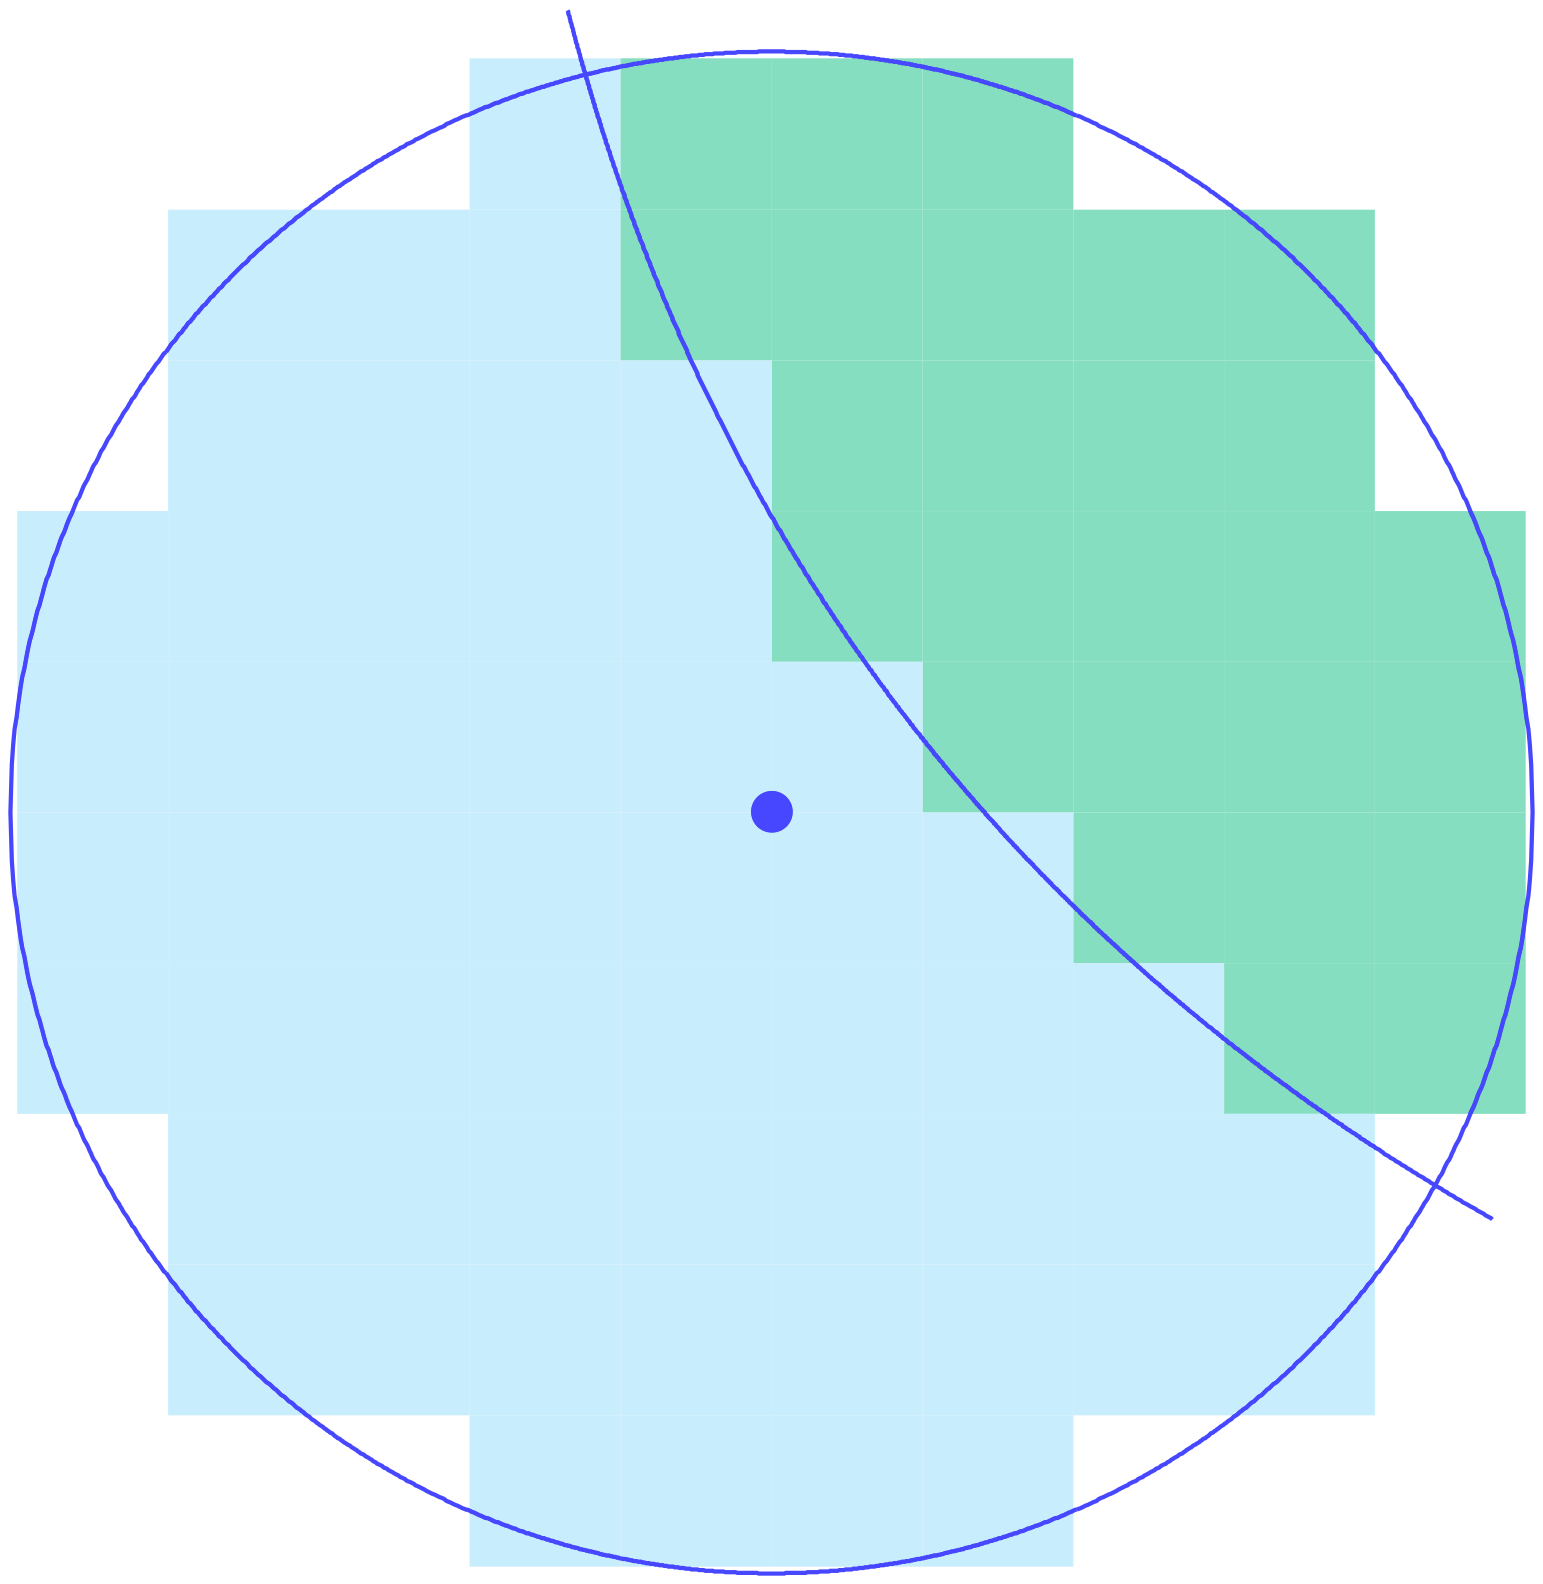
\includegraphics[scale=0.57]{media/2-shabaka/1-vor/dem2.png}
\label{fig:vor2}}
\subfigure[]{%
		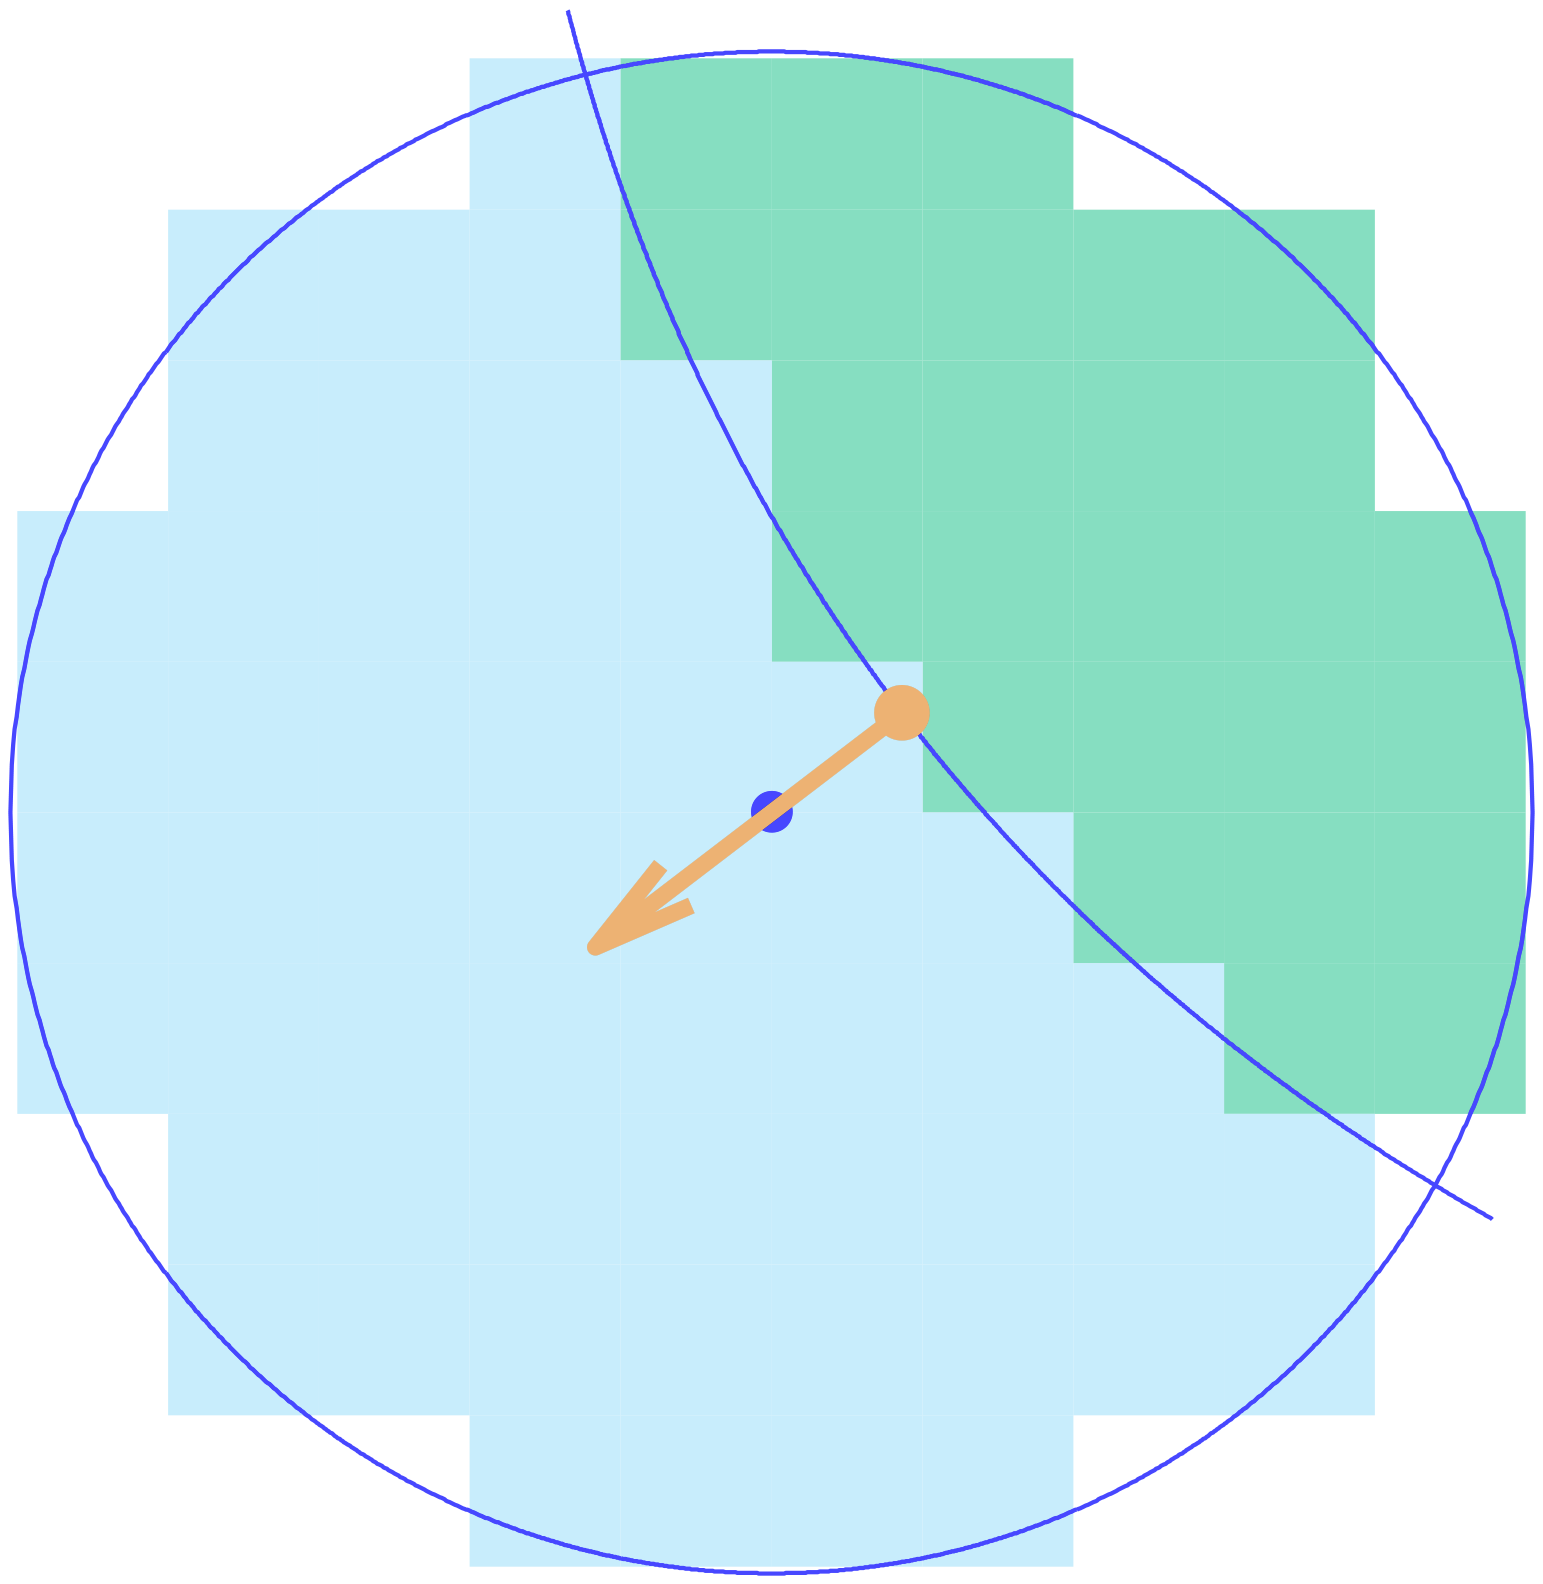
\includegraphics[scale=0.57]{media/2-shabaka/1-vor/dem3.png}
\label{fig:vor3}}
\subfigure[]{%
		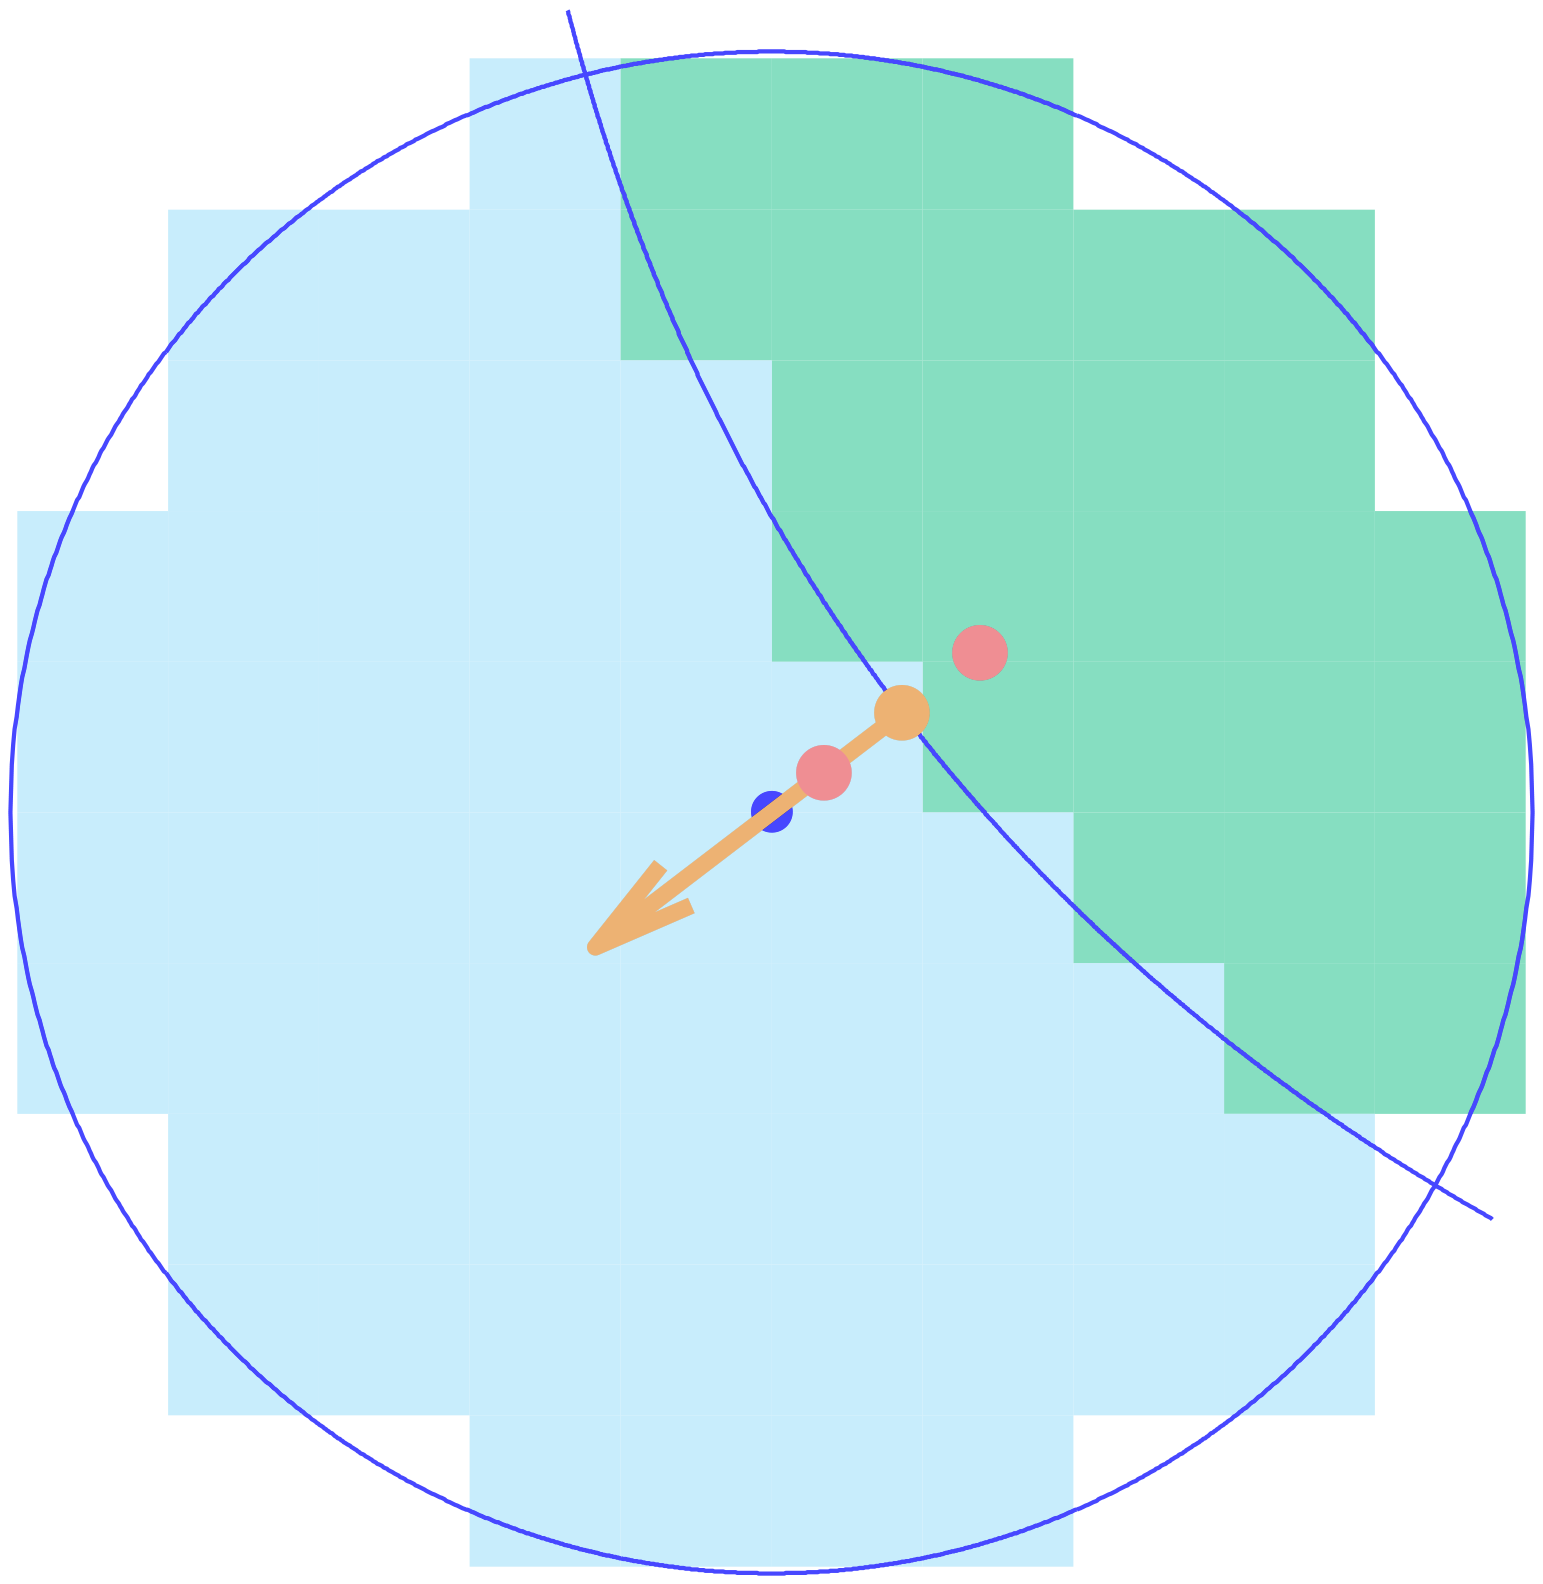
\includegraphics[scale=0.57]{media/2-shabaka/1-vor/dem4.png}
\label{fig:vor4}}
%
\caption{(a) Sample window of segmented image, (b) interface approximation, (c) point/normal placement, and d) Voronoi site placement}
\label{fig:vor}
\end{figure}

\begin{figure}[ht]
\centering
\subfigure[]{%
		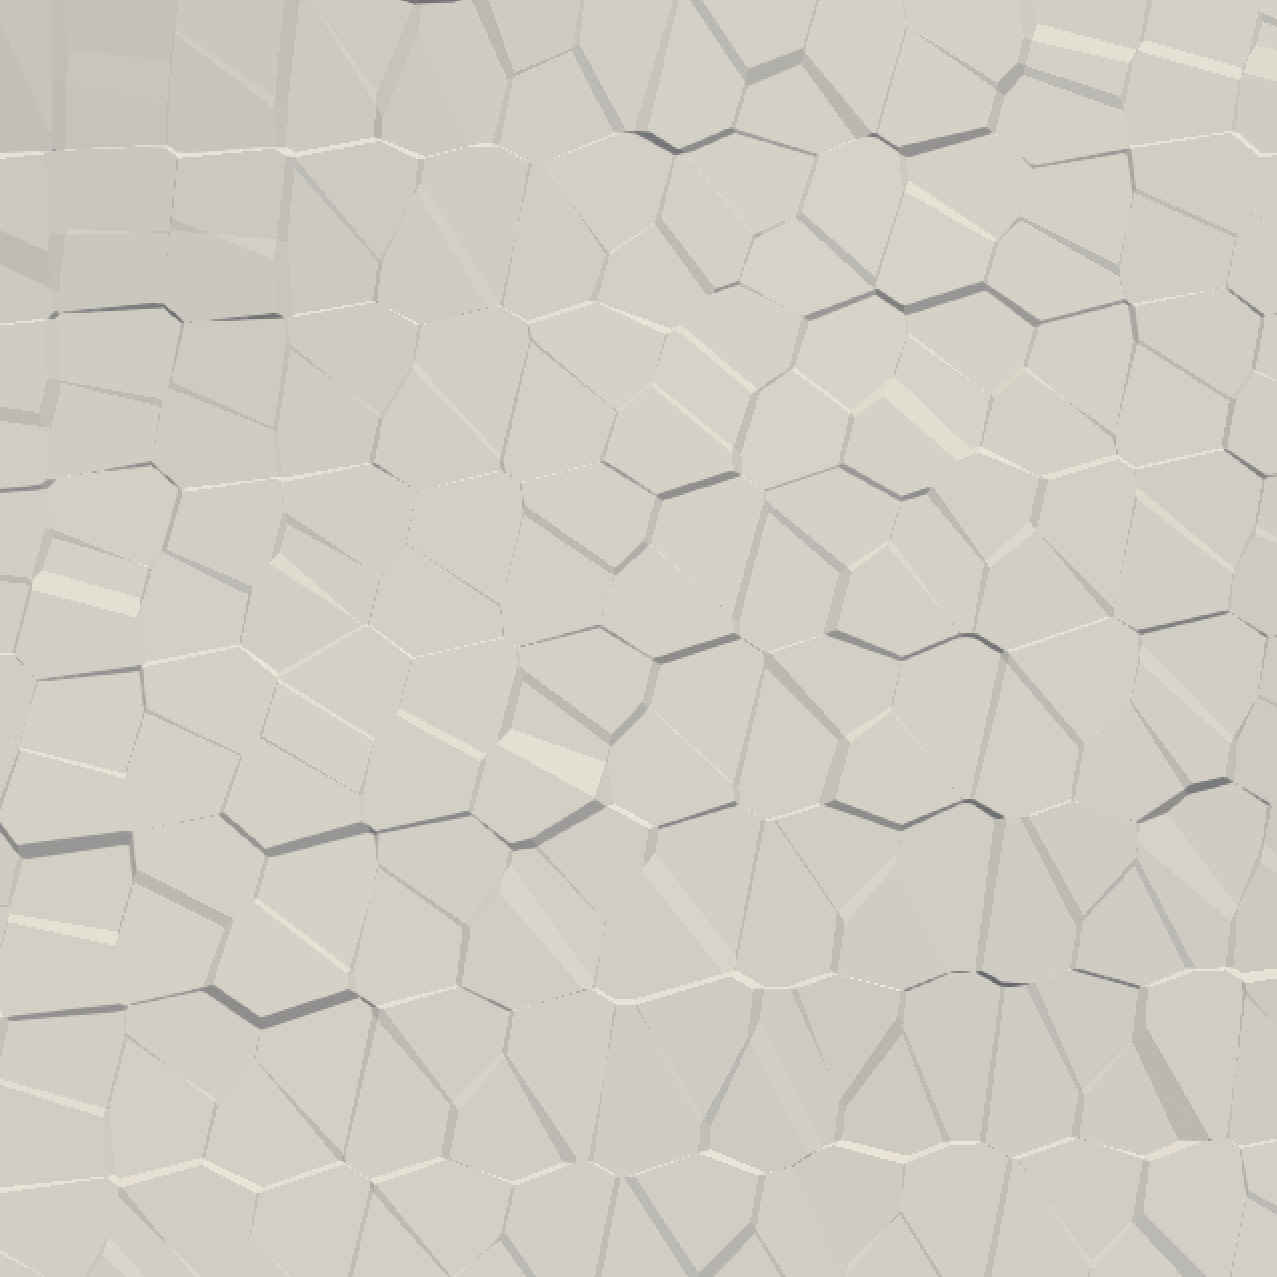
\includegraphics[scale=0.083]{media/2-shabaka/3-clean-zoom/1-init-zoom.png}
\label{fig:cross1-1}}		
\subfigure[]{%
		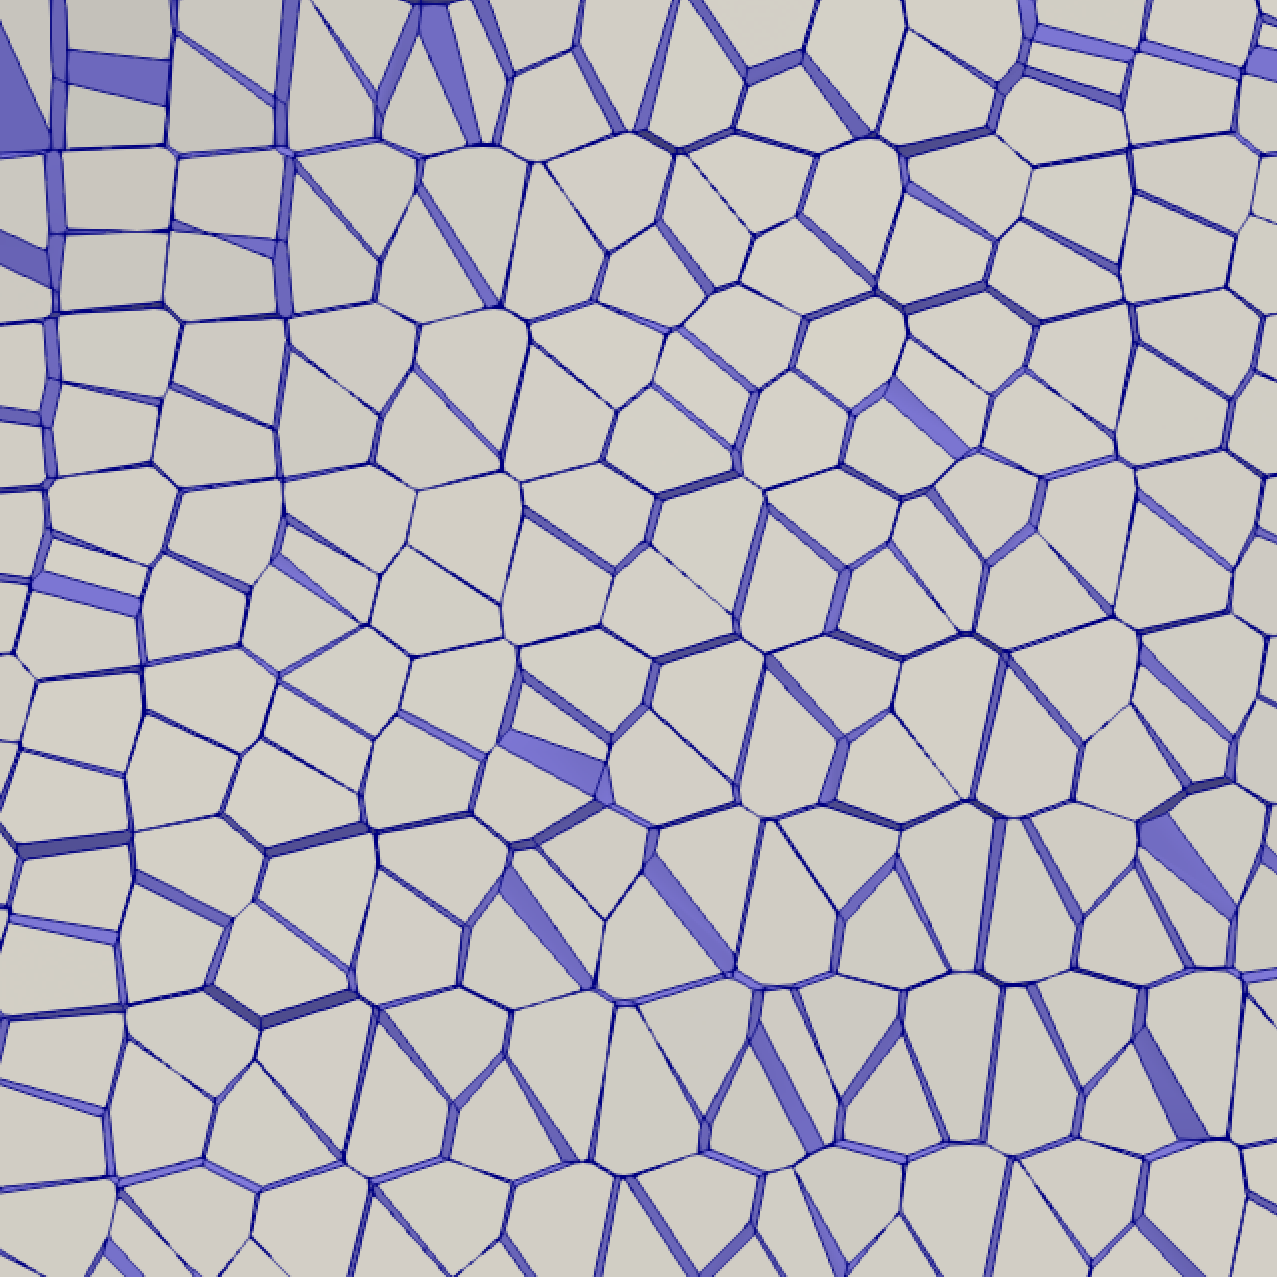
\includegraphics[scale=0.083]{media/2-shabaka/3-clean-zoom/2-badfacets-zoom.png}
\label{fig:cross1-2}}		
\subfigure[]{%
		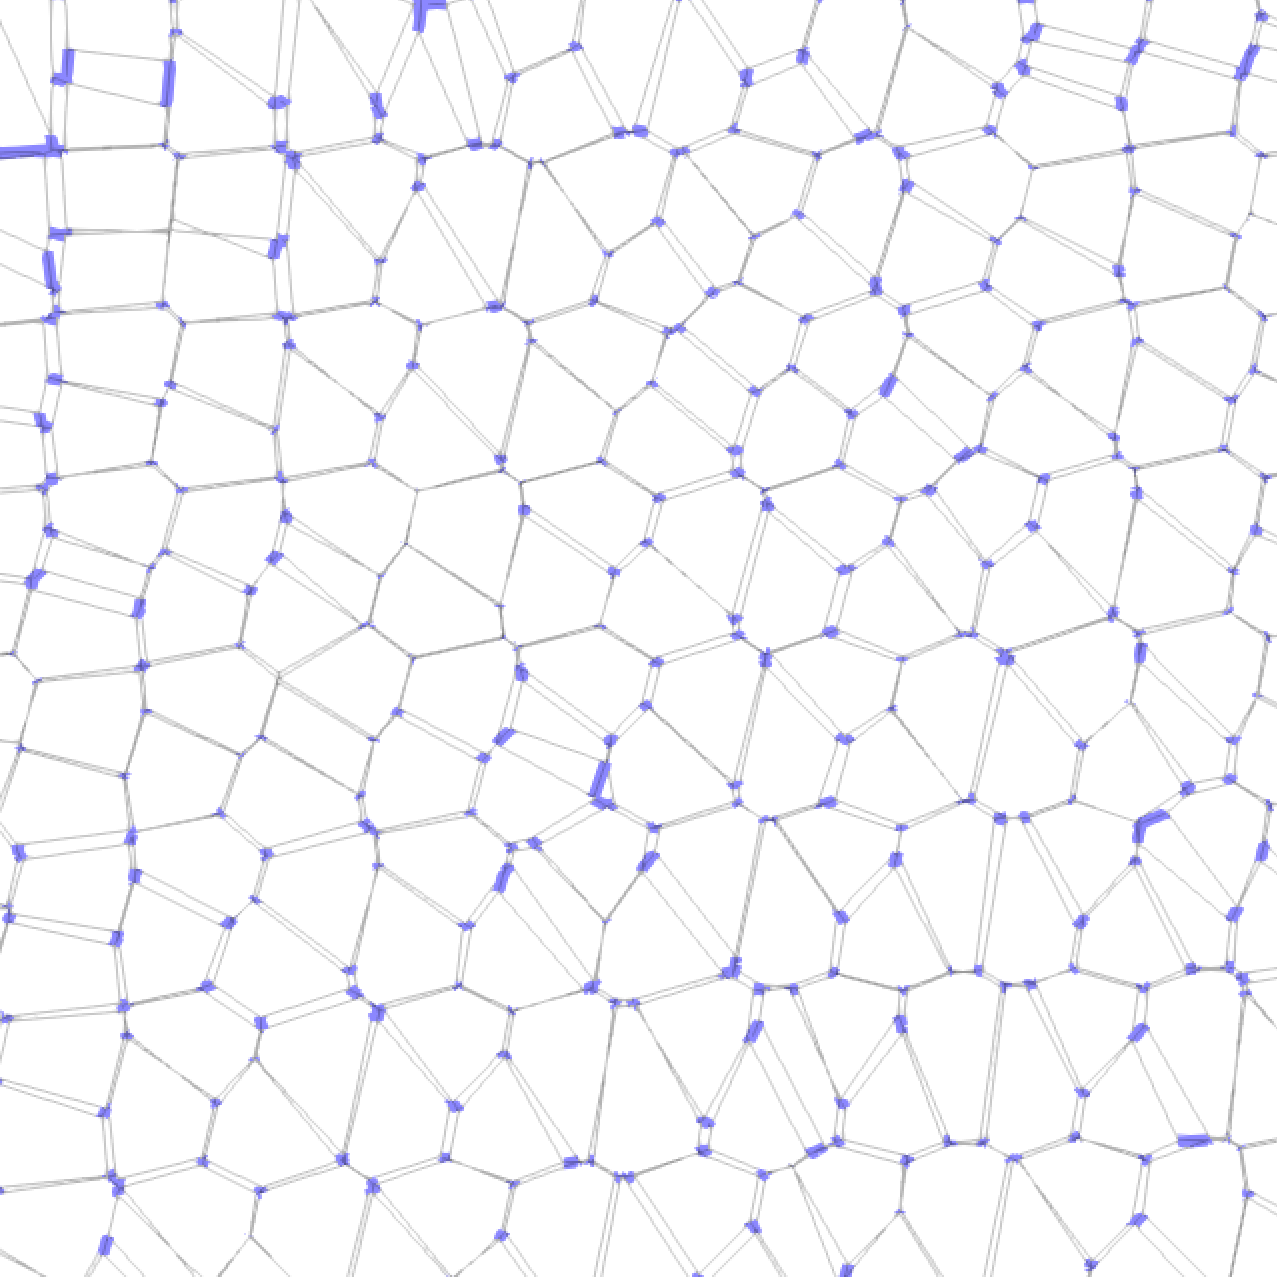
\includegraphics[scale=0.083]{media/2-shabaka/3-clean-zoom/3-badsegs-zoom.png}		
\label{fig:cross1-3}}					
\subfigure[]{%
		
\includegraphics[scale=0.083]{media/2-shabaka/3-clean-zoom/4-fine-zoom.png}
\label{fig:cross1-4}}				
%
\caption{Clean-up of undesirable ``cross-talk'' facets for a surface patch: (a) initial surface following Voronoi-based surface reconstruction, (b) identification of ``cross-talk'' facets, (c) identification of edges to be collapsed, (d) final cleaned surface.}
\label{fig:cross1}
\end{figure}

\begin{figure}[ht]
\centering
\subfigure[]{%
		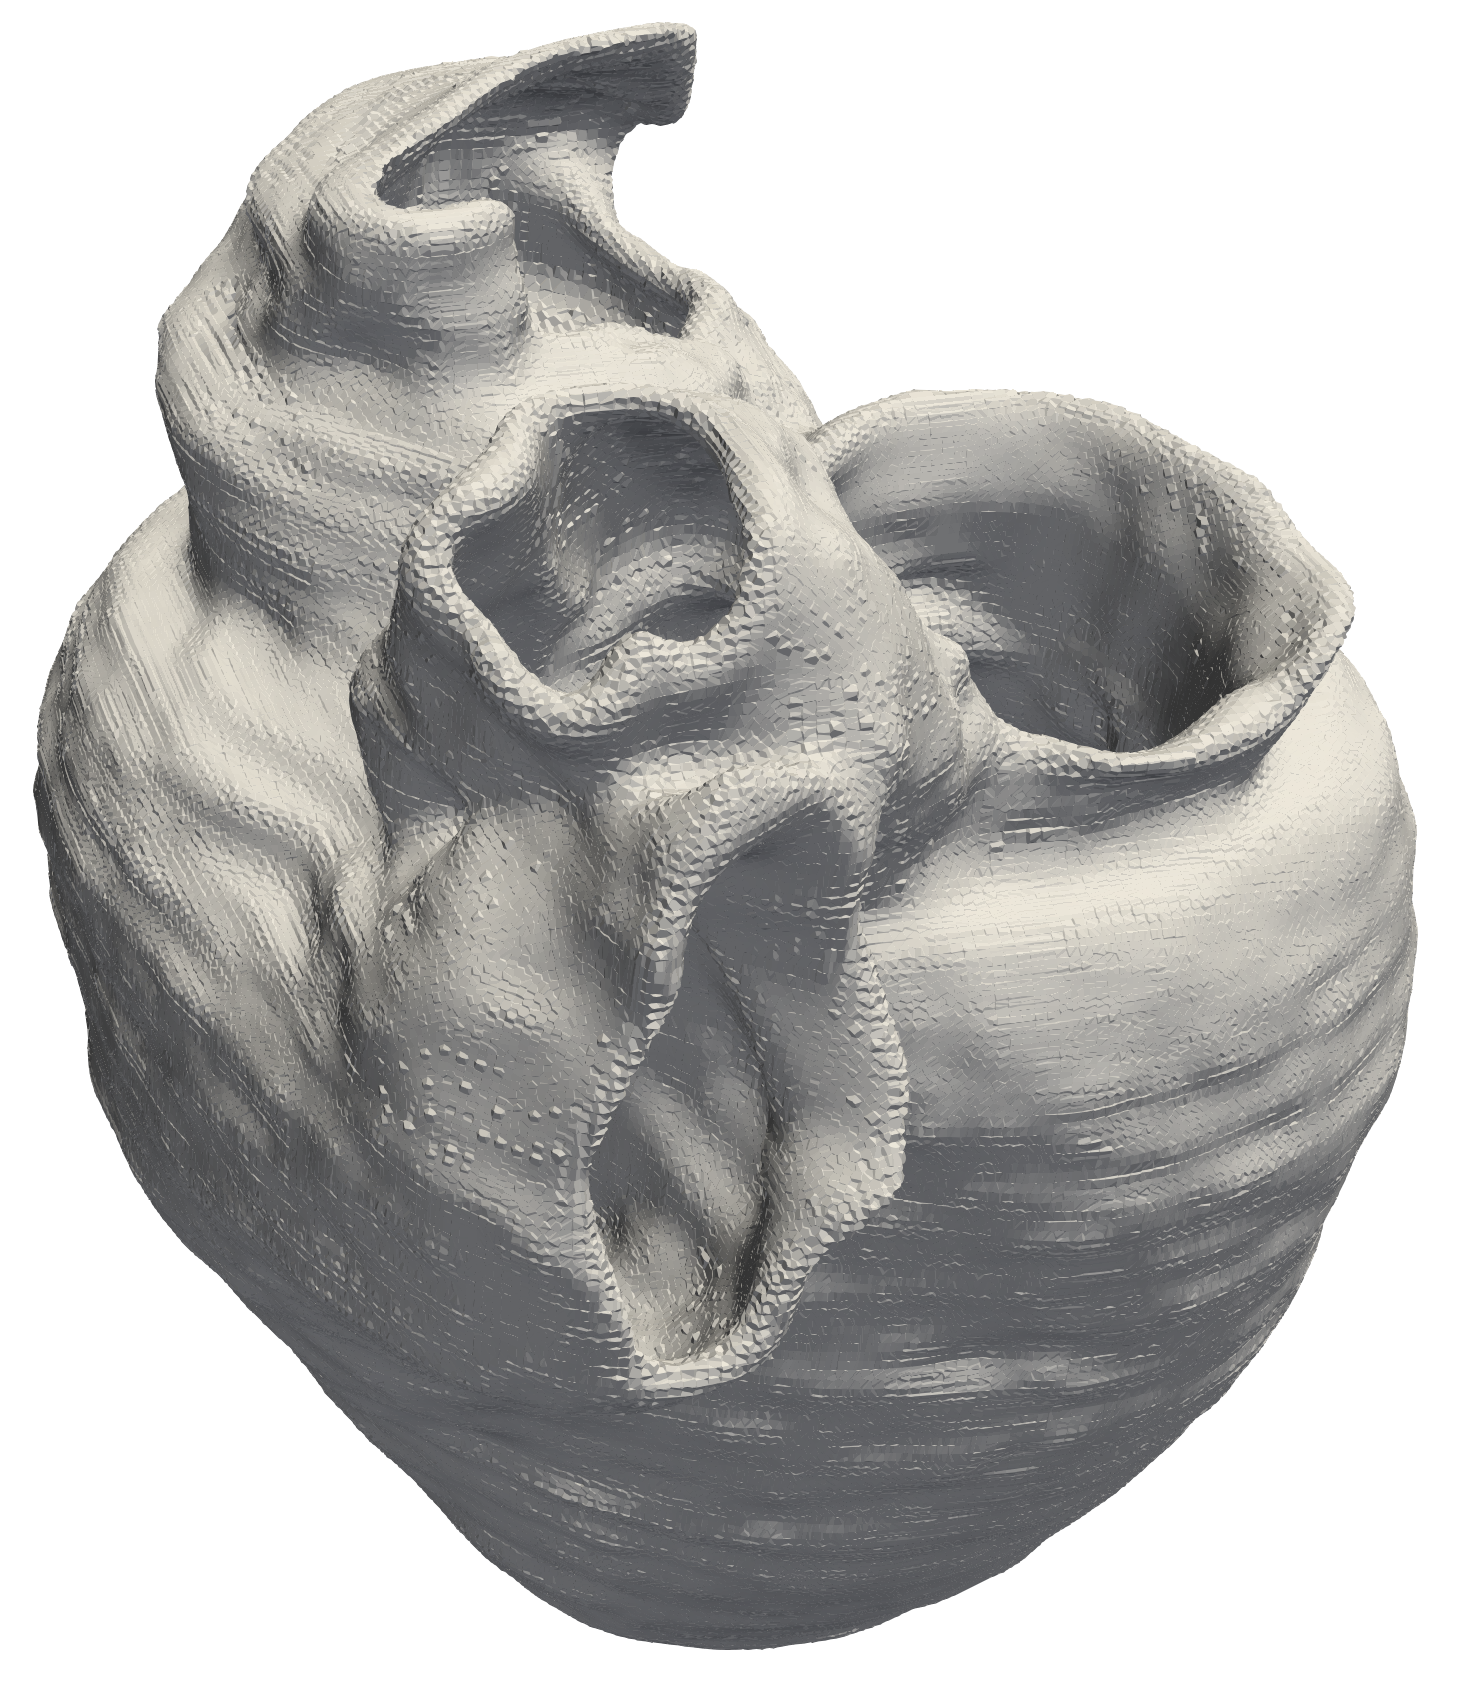
\includegraphics[scale=0.07]{media/2-shabaka/4-clean/1-init.png}
\label{fig:cross2-1}}		
\subfigure[]{%
		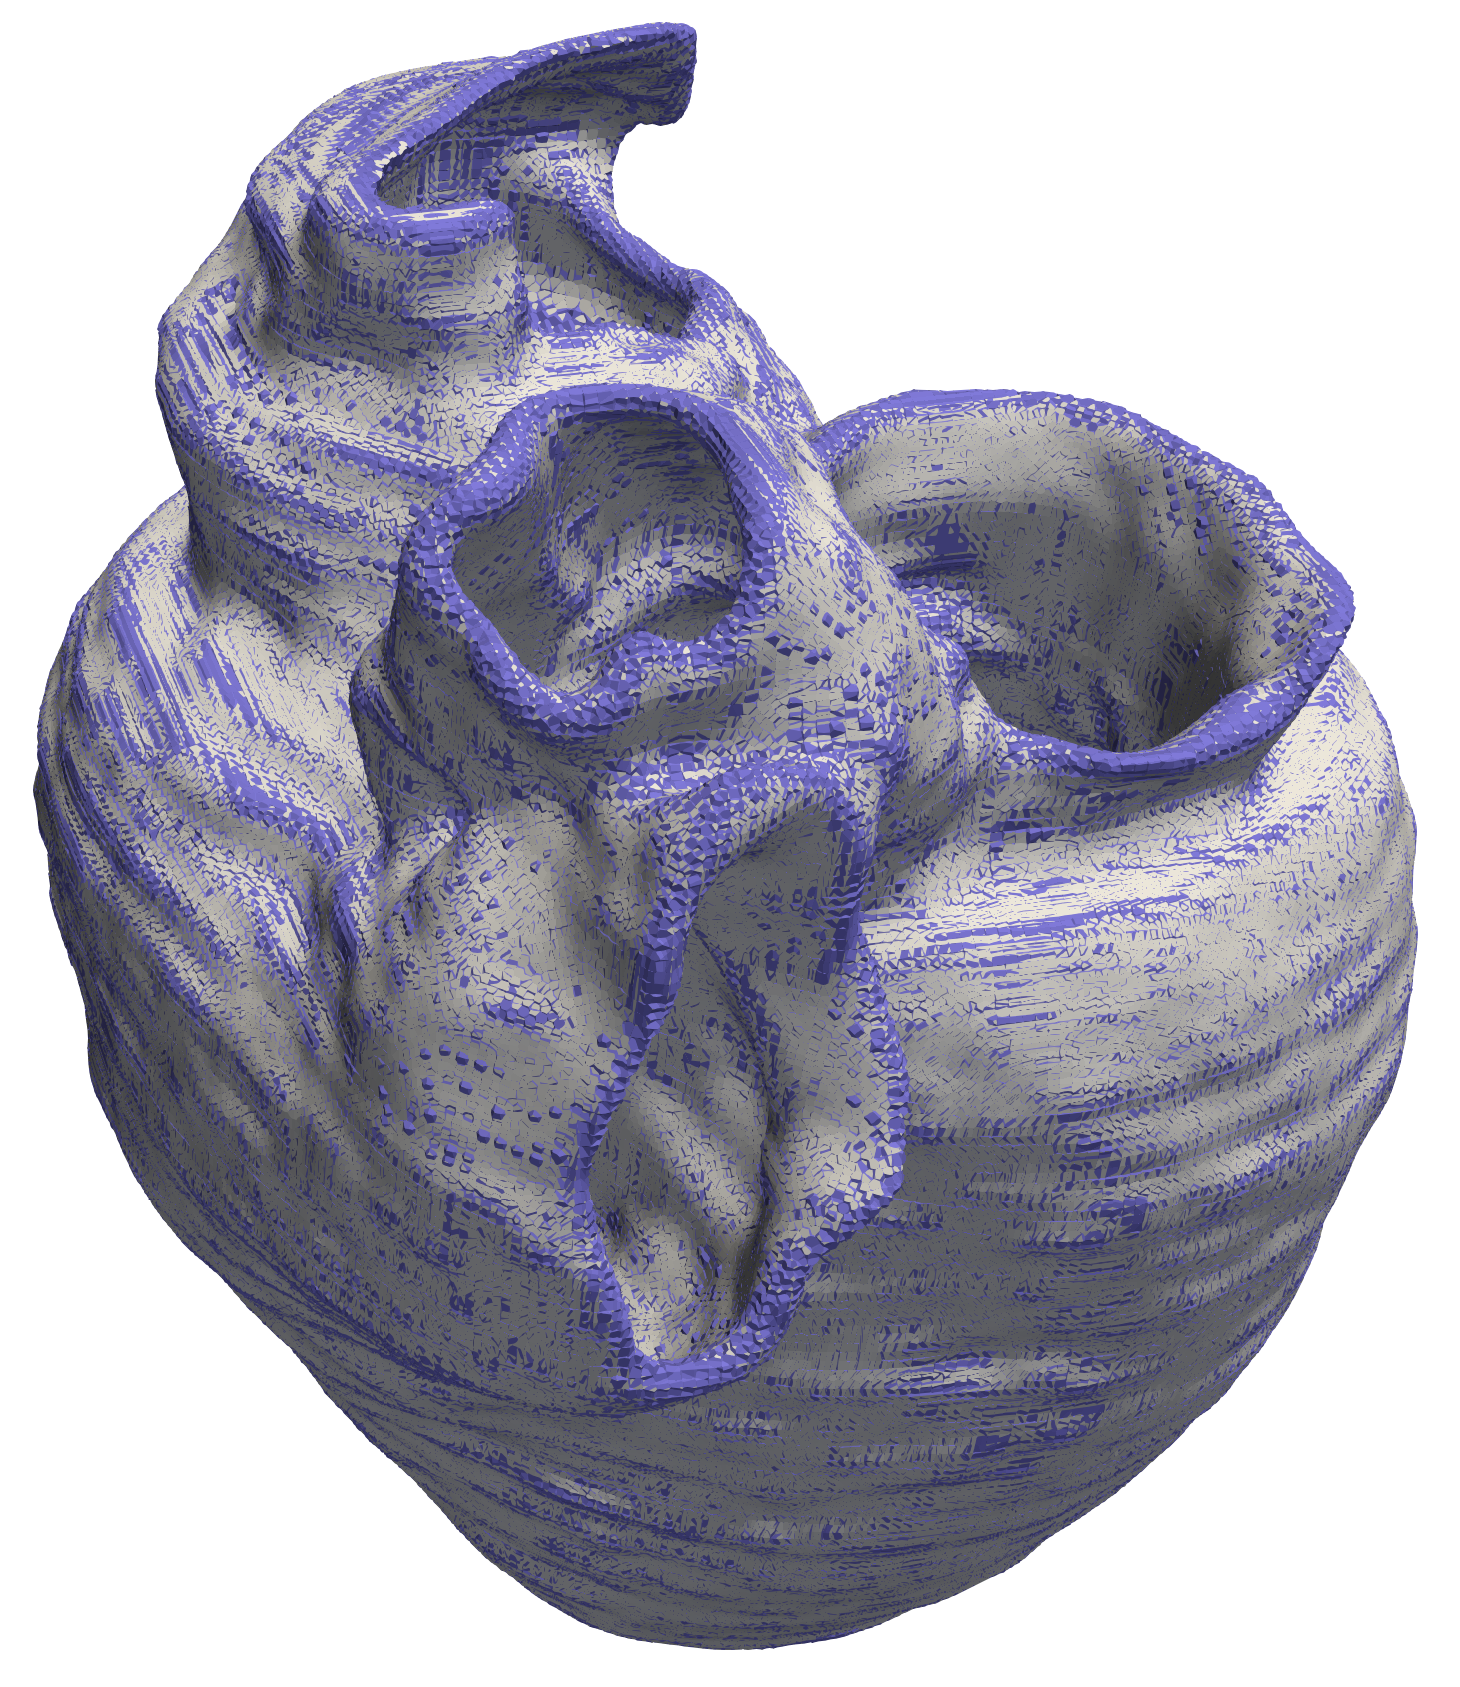
\includegraphics[scale=0.07]{media/2-shabaka/4-clean/2-badfacets.png}
\label{fig:cross2-2}}		
\subfigure[]{%
		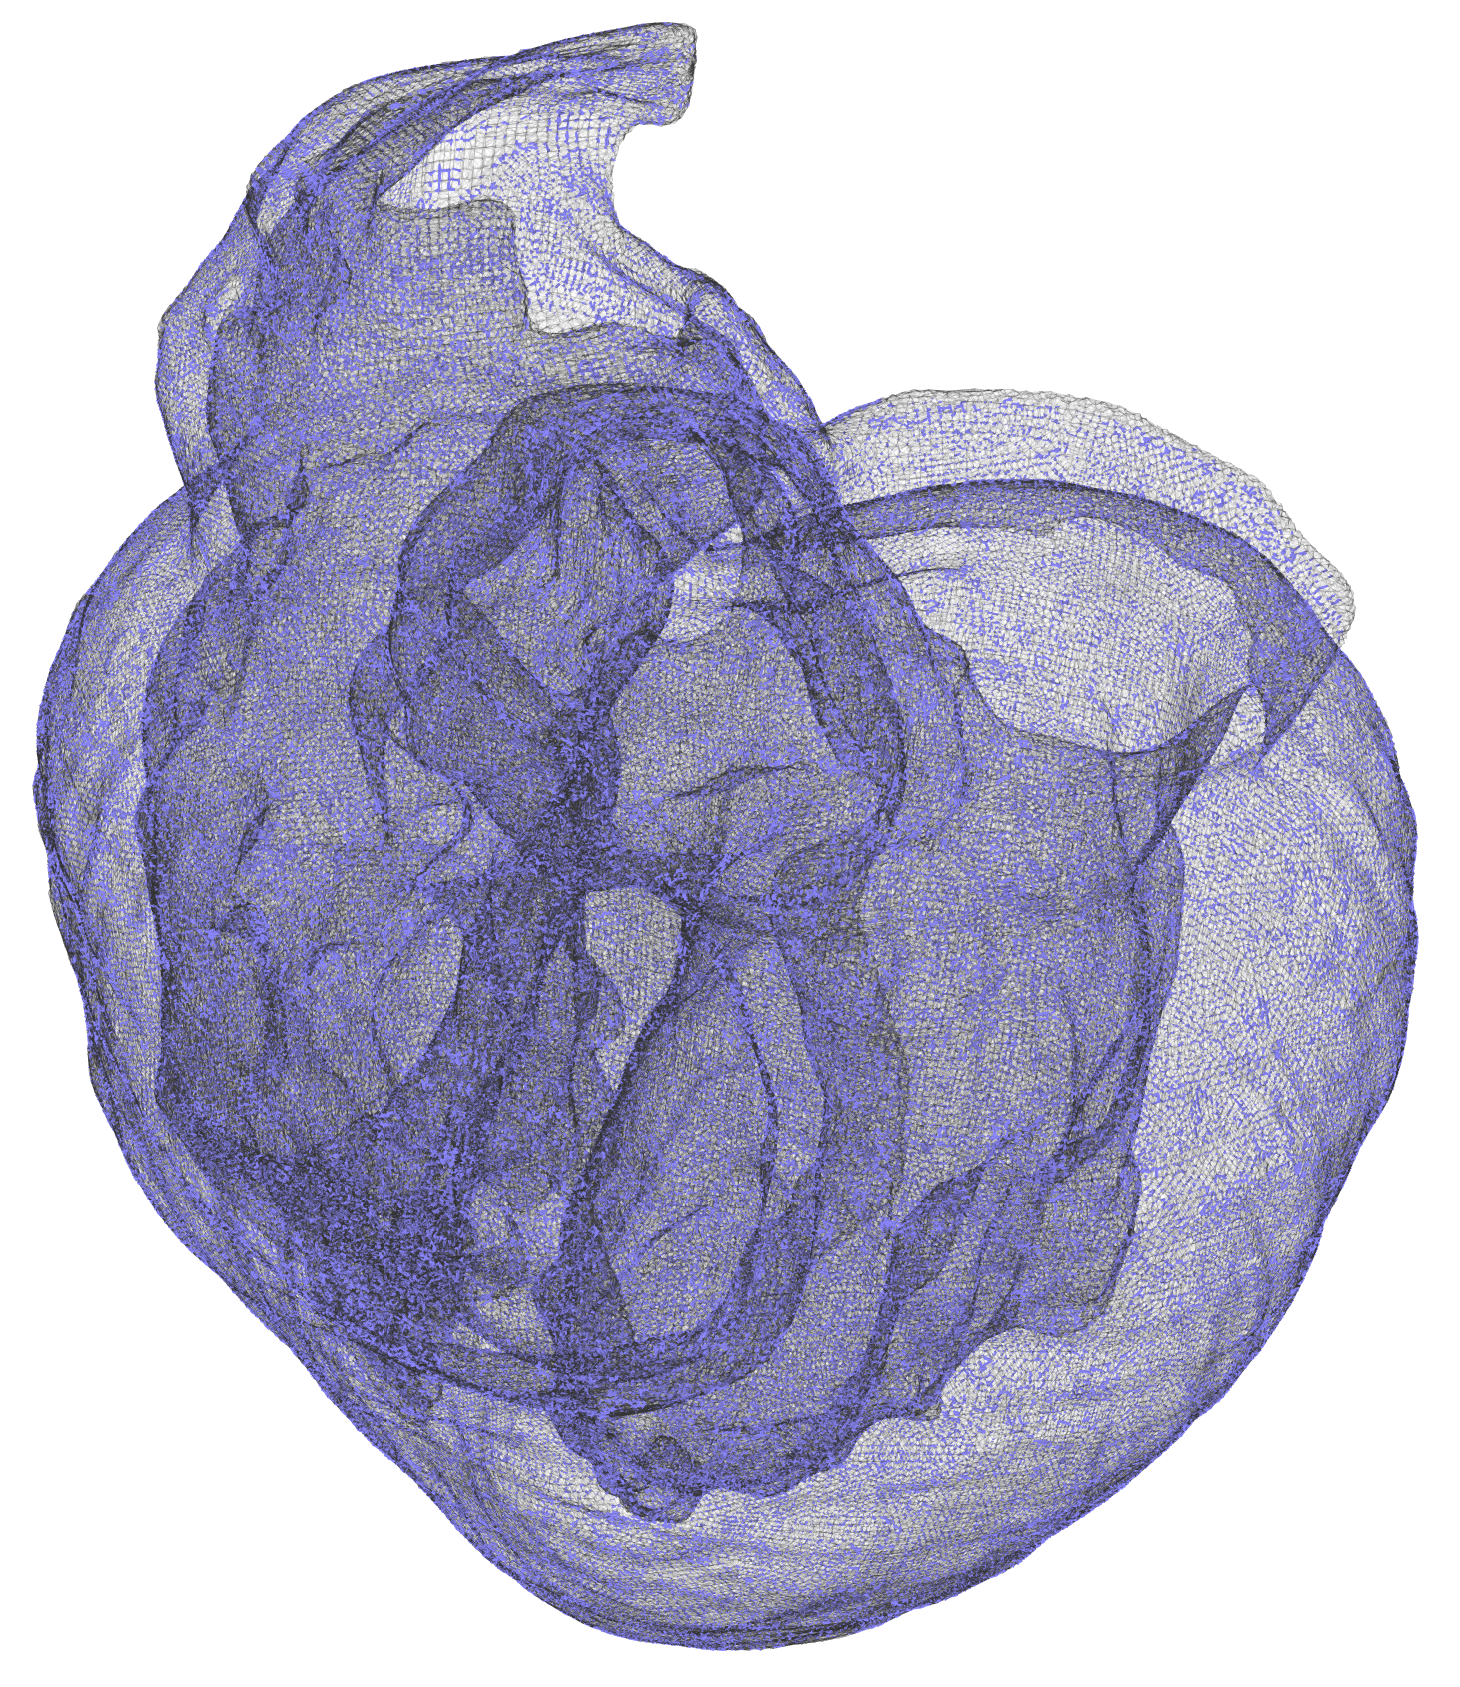
\includegraphics[scale=0.07]{media/2-shabaka/4-clean/3-badsegs.png}	
\label{fig:cross2-3}}						
\subfigure[]{%
		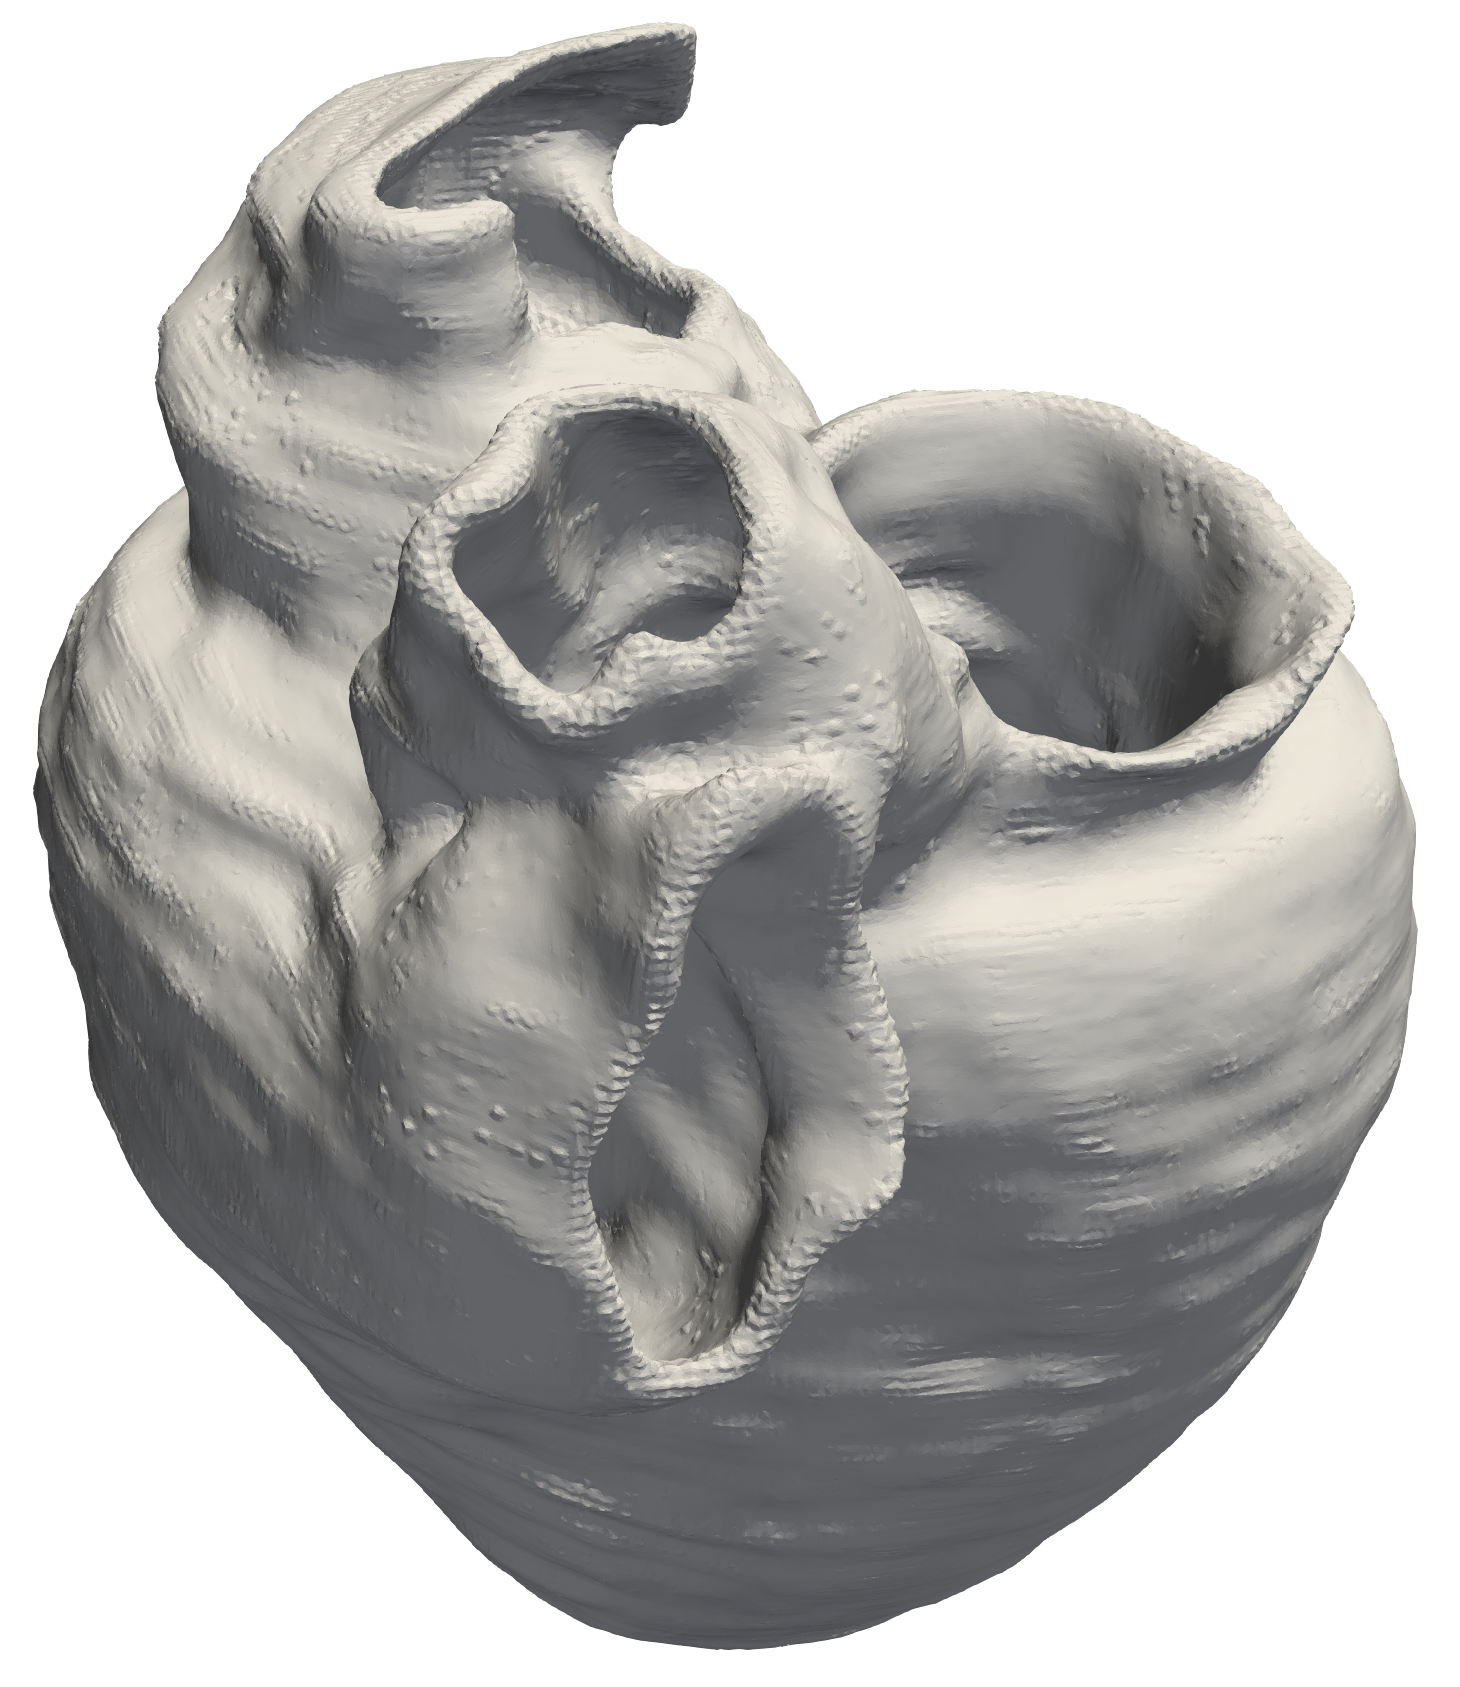
\includegraphics[scale=0.07]{media/2-shabaka/4-clean/4-fine.png}		
\label{fig:cross2-4}}		
%
\caption{Clean-up of undesirable ``cross-talk'' facets for surface of \textit{ex-vivo} human heart: (a) initial surface following Voronoi-based surface reconstruction, (b) identification of ``cross-talk'' facets, (c) identification of edges to be collapsed, (d) final cleaned surface.}
\label{fig:cross2}
\end{figure}

\begin{figure}[ht!]
\centering
\subfigure[]{%
		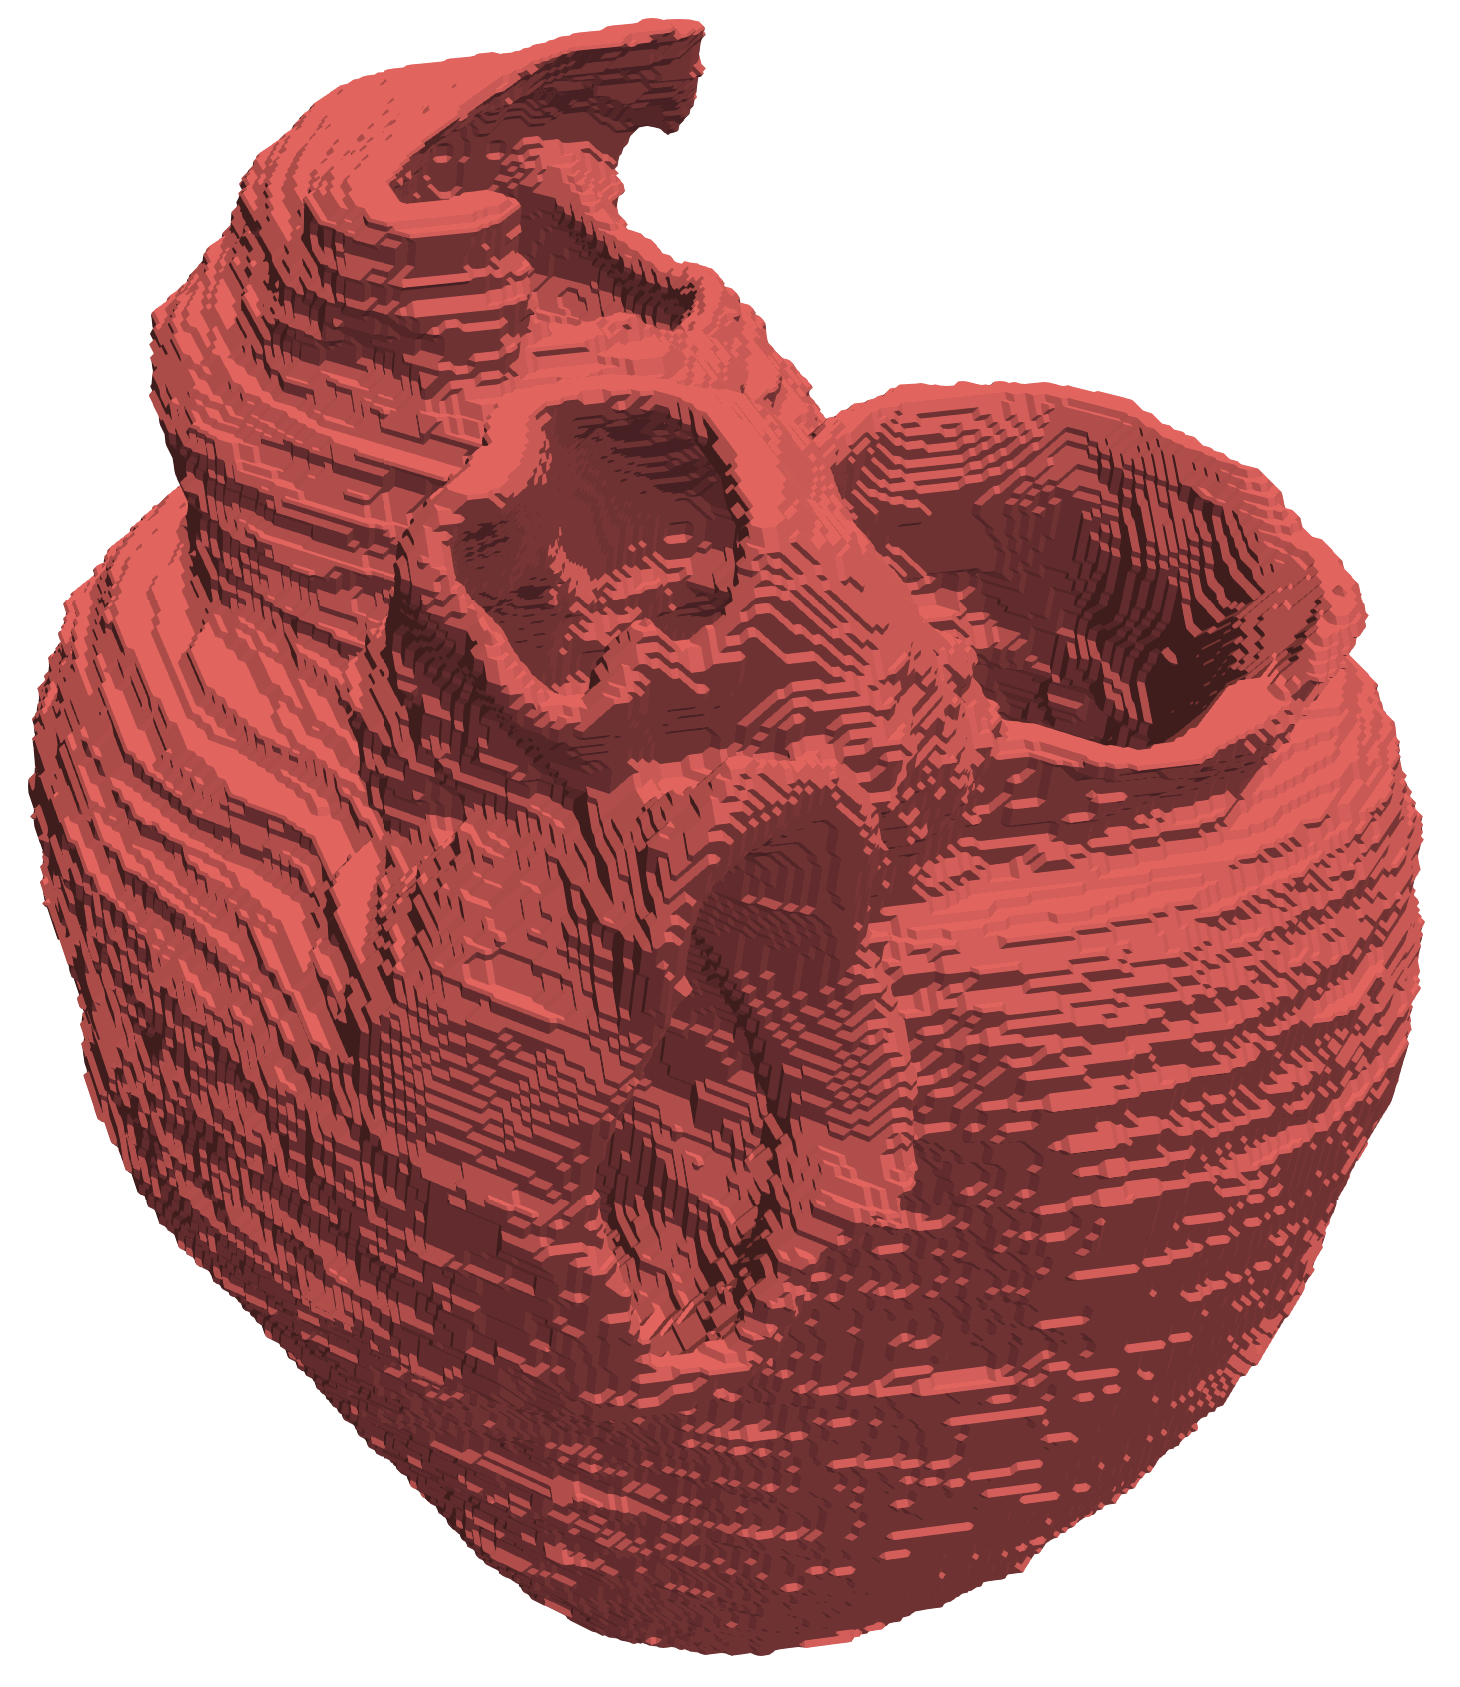
\includegraphics[scale=0.092]{media/2-shabaka/2-surf/1-seg.png}
\label{fig:shabakaseq1}}
\subfigure[]{%
		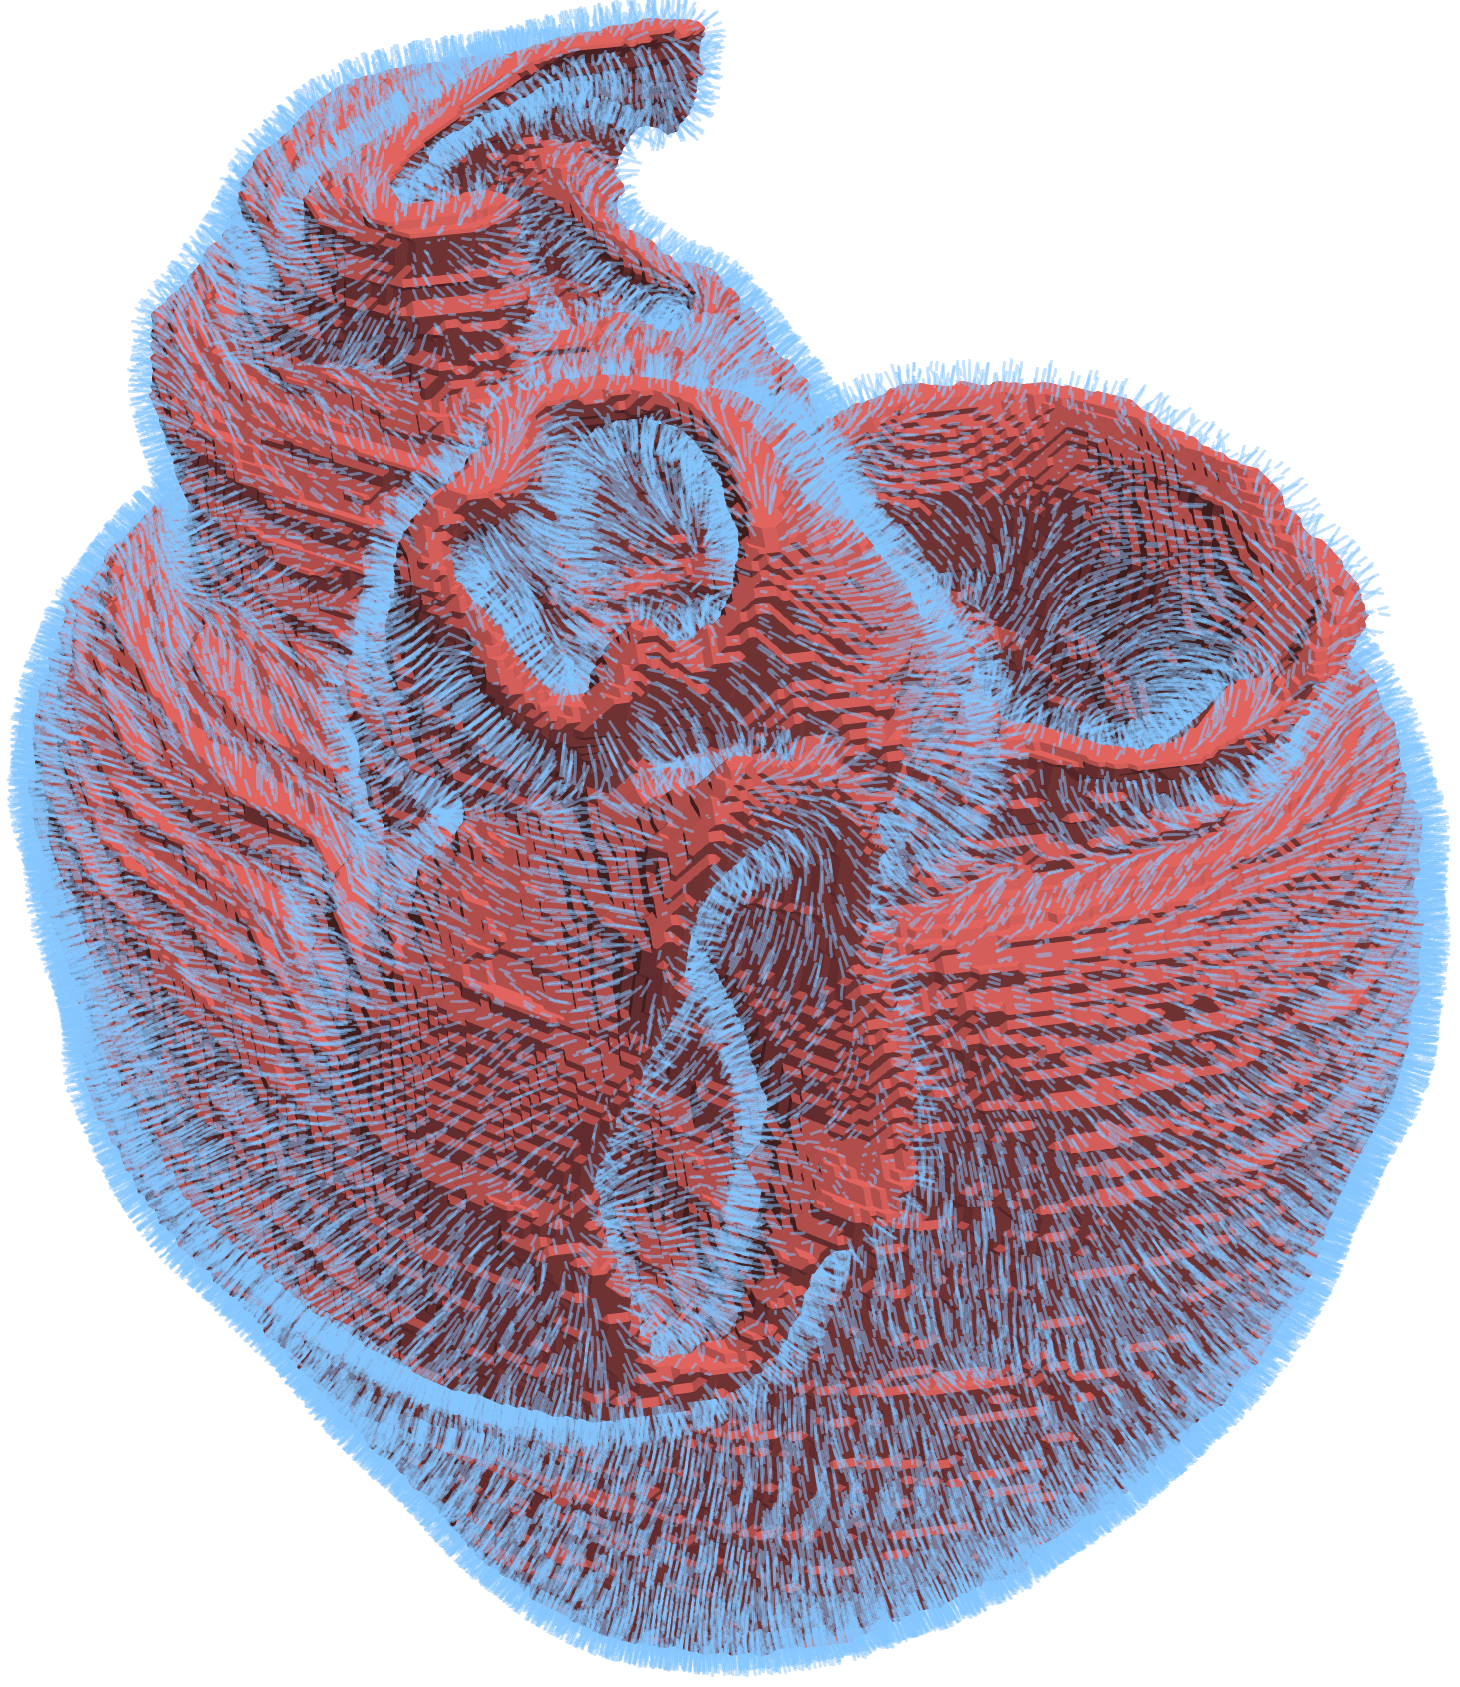
\includegraphics[scale=0.092]{media/2-shabaka/2-surf/2-normals.png}
\label{fig:shabakaseq2}}
\subfigure[]{%
		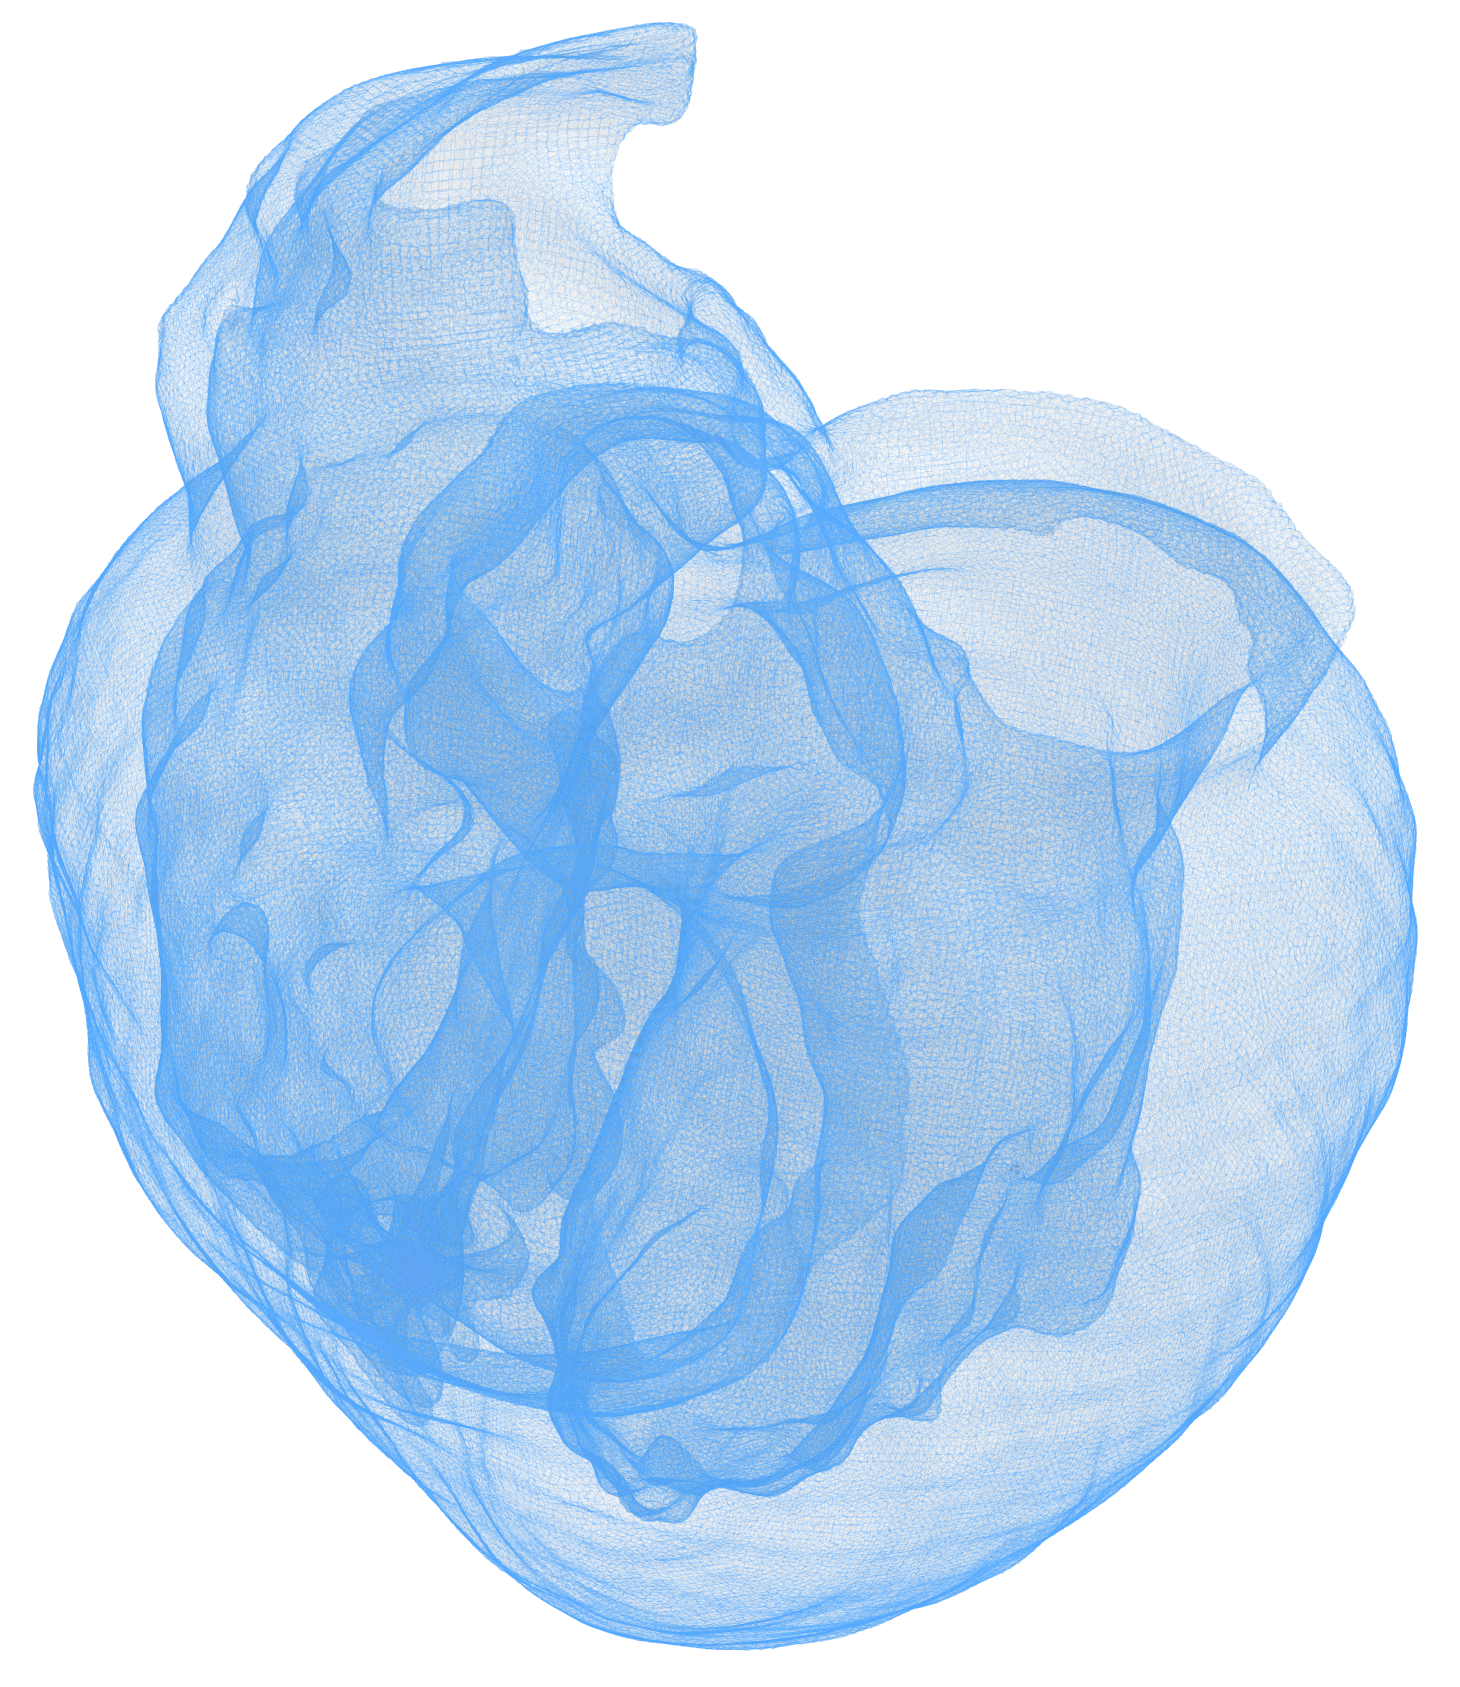
\includegraphics[scale=0.092]{media/2-shabaka/2-surf/3-ptcloud.png}
\label{fig:shabakaseq3}}
\subfigure[]{%
		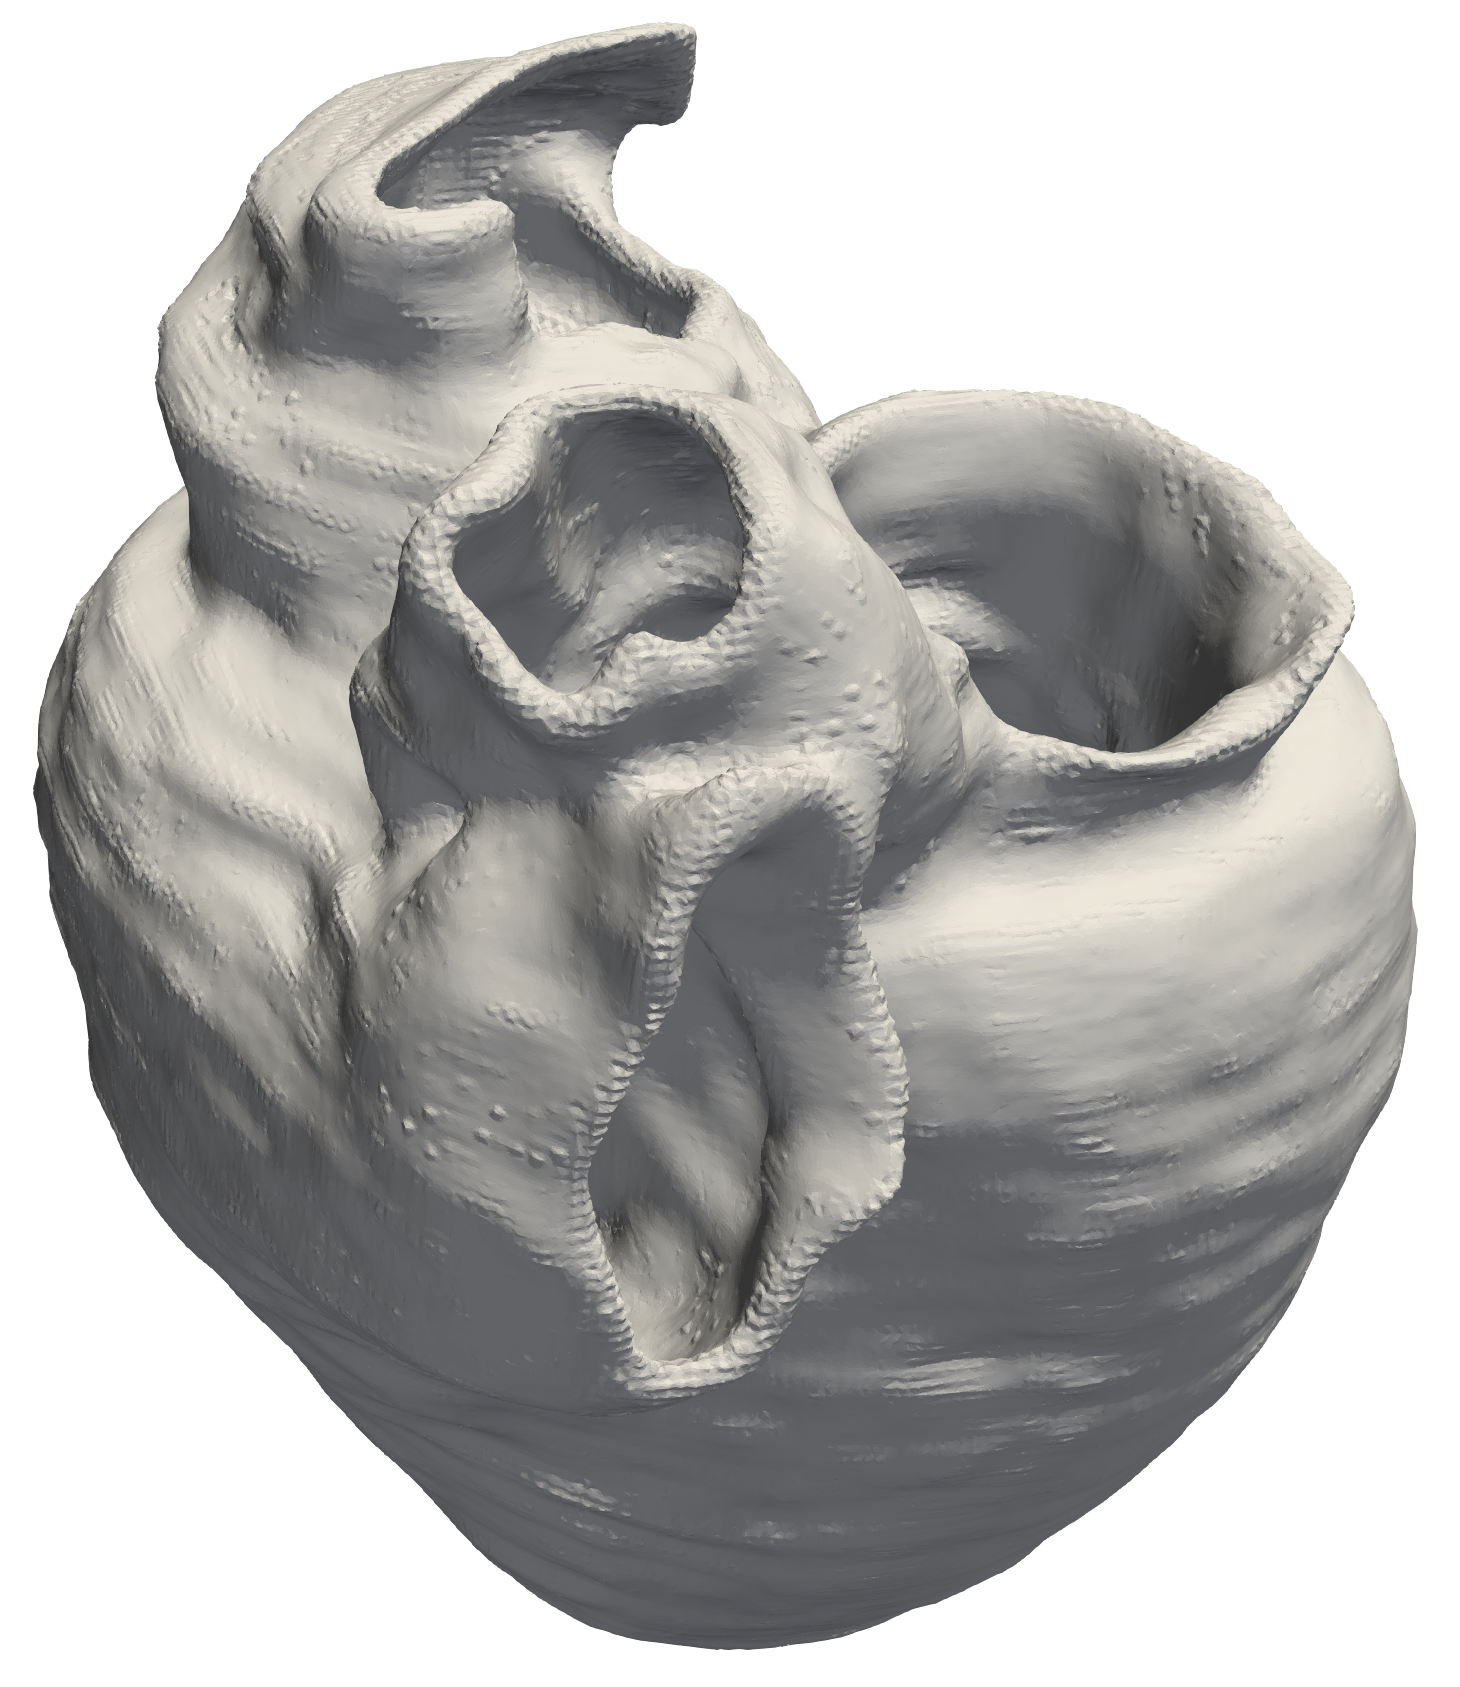
\includegraphics[scale=0.092]{media/2-shabaka/2-surf/4-finesurf.png}
\label{fig:shabakaseq4}}
\subfigure[]{%
		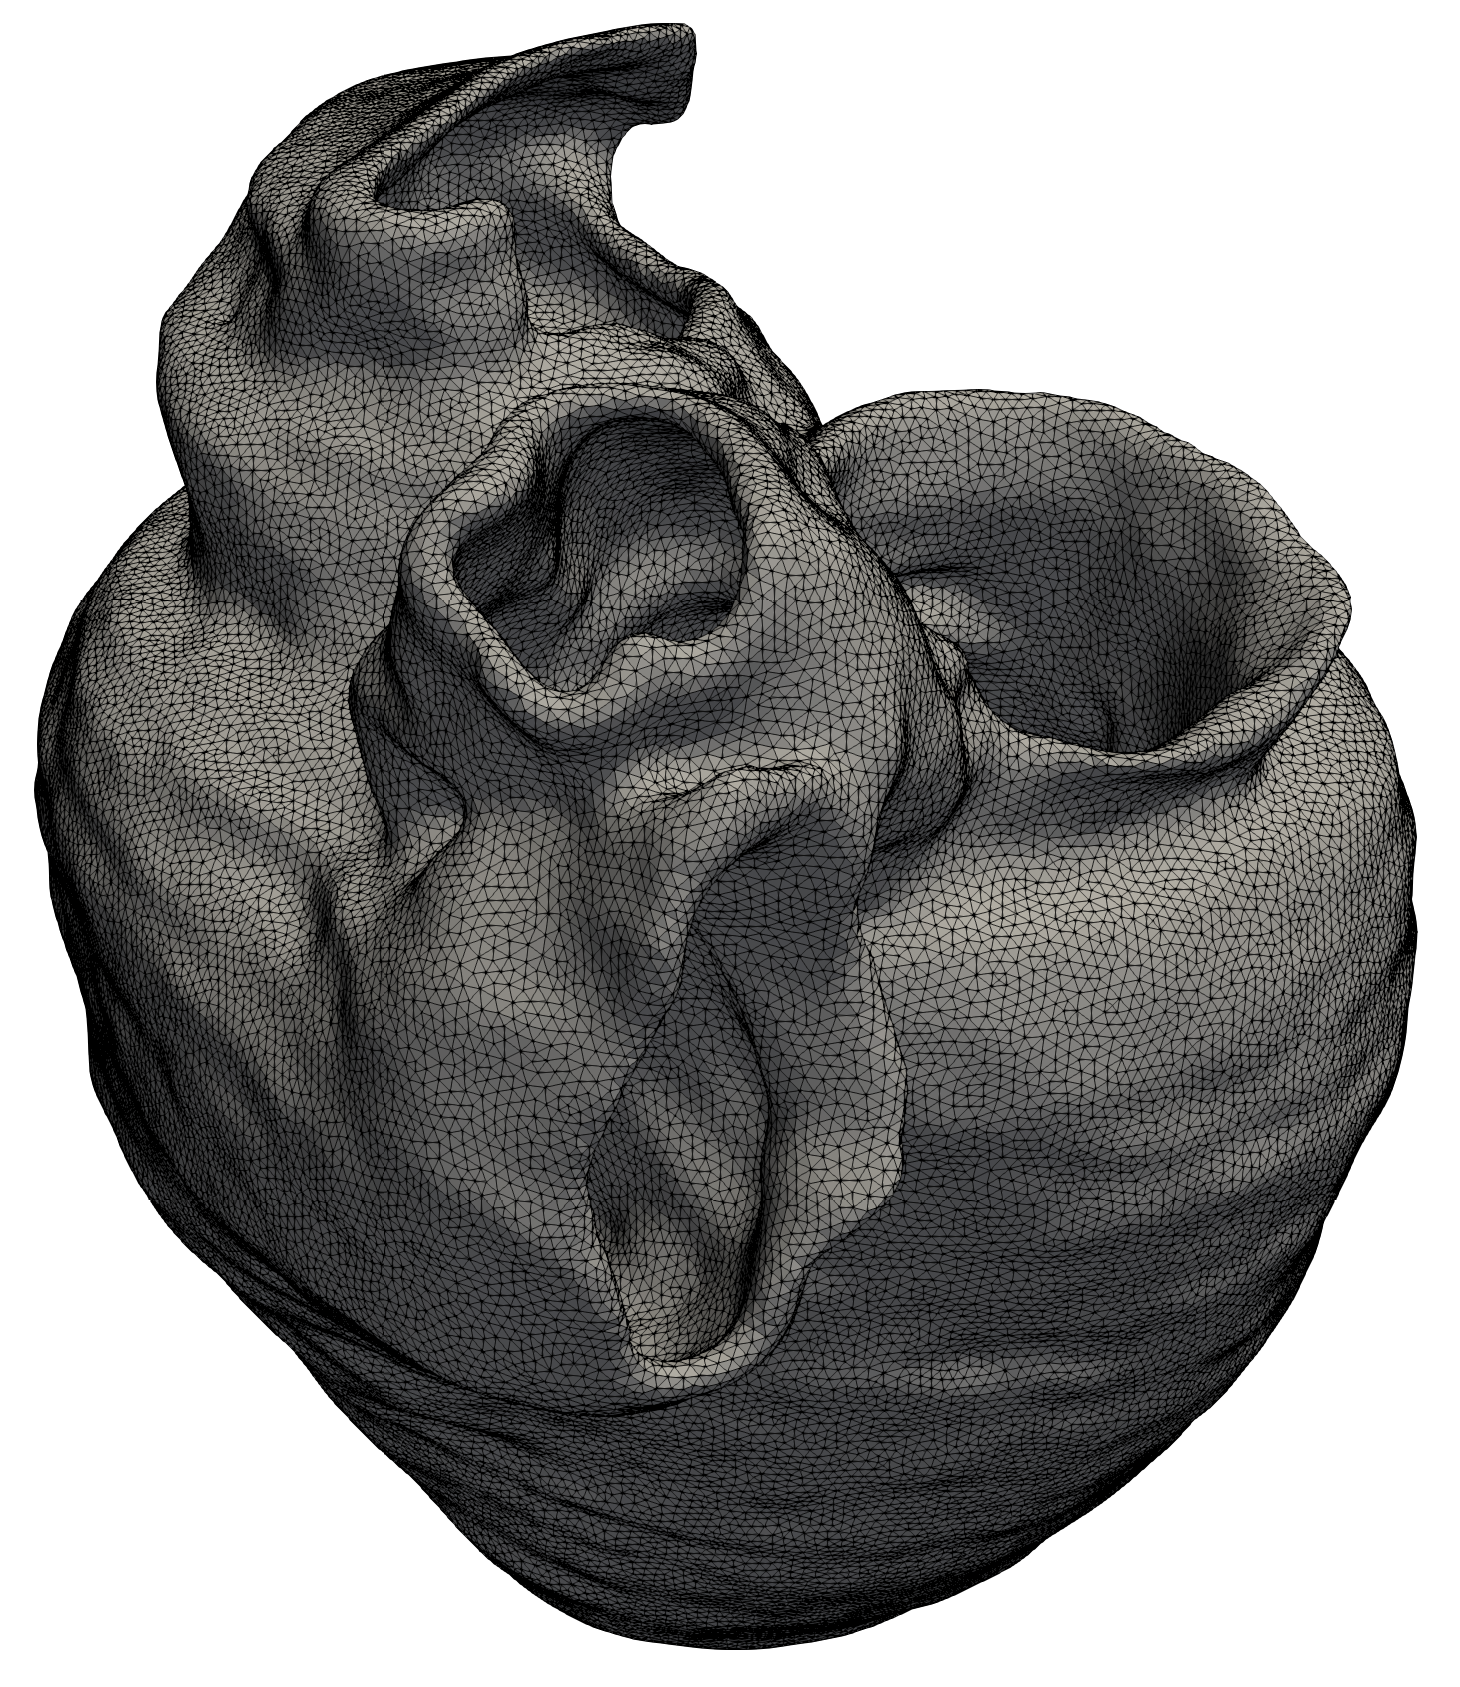
\includegraphics[scale=0.092]{media/2-shabaka/2-surf/5-surf.png}
\label{fig:shabakaseq5}}
%
\caption{(a) Segmented image, (b) point/normal placement, (c) oriented point cloud (normals not shown), c) cleaned surface mesh generated from Voronoi partition (edges not shown), and d) final decimated surface}
\label{fig:shabakaseq}
\end{figure}

\begin{figure}[ht!]
\centering
\vspace{2.5mm}
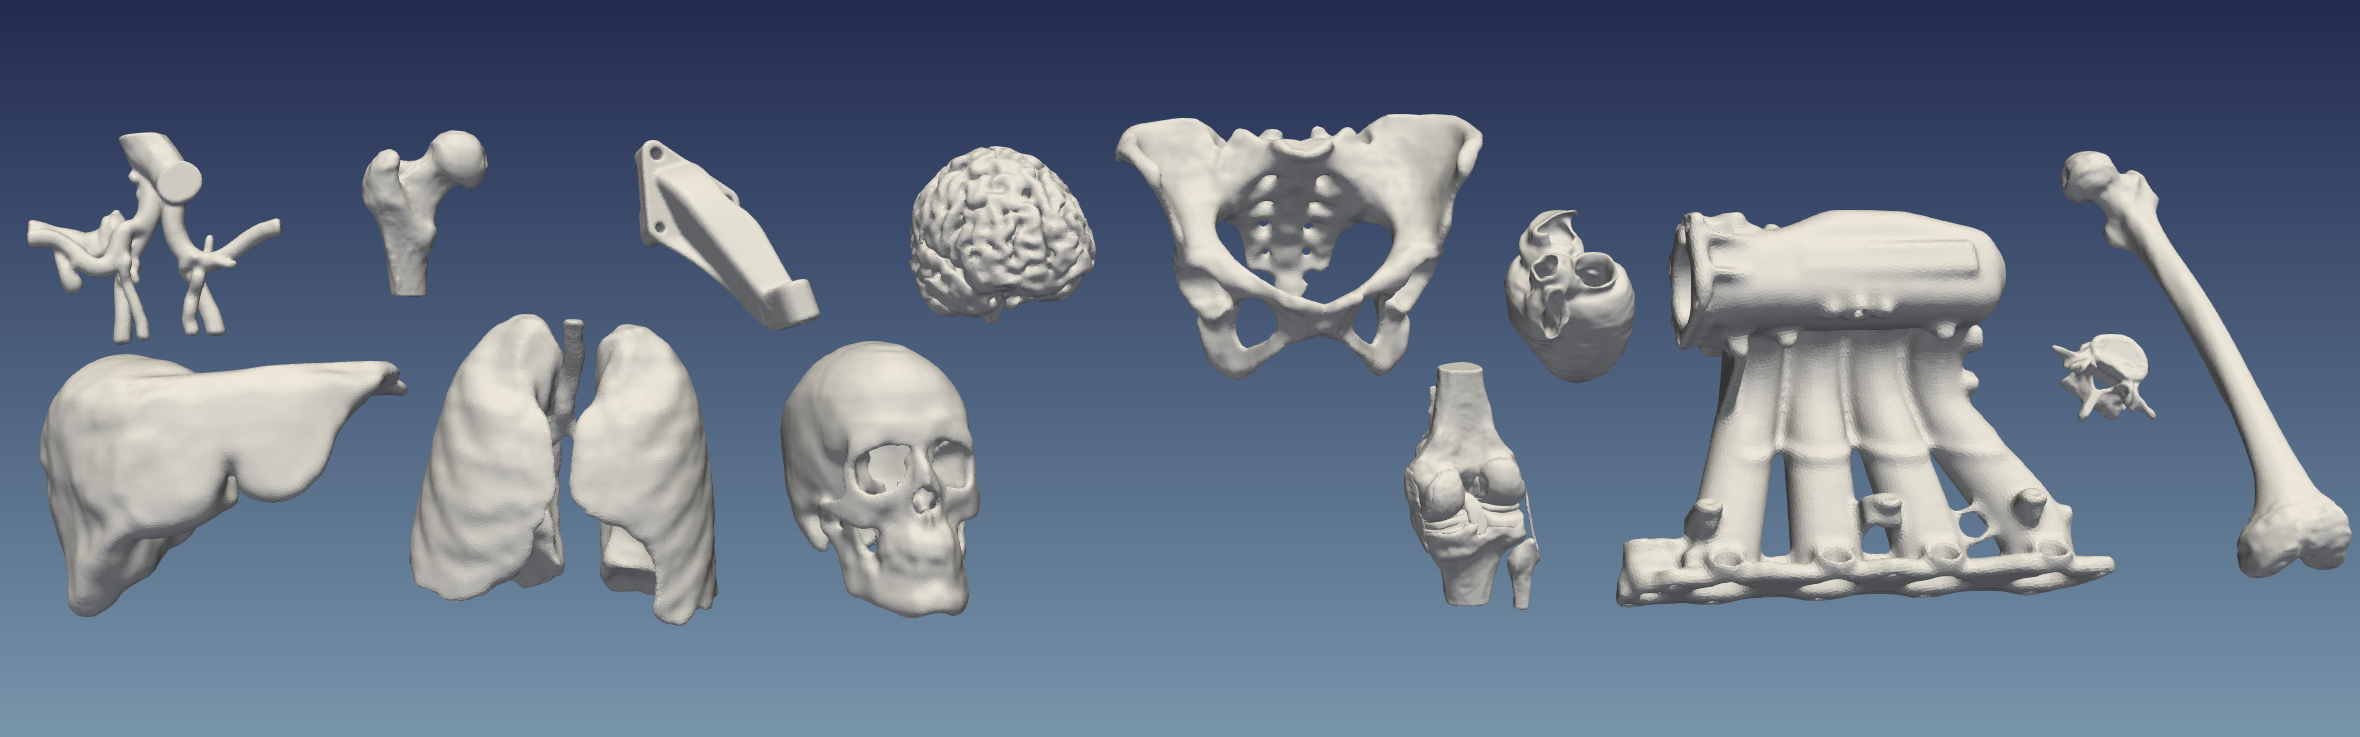
\includegraphics[width=1.0\textwidth]{media/2-shabaka/2-surf/6-showcase.png}
\caption{Suite of example surfaces generated from image data.}
\label{fig:showcase}
\end{figure}

\begin{figure}[ht!]
\centering
\vspace{2.5mm}
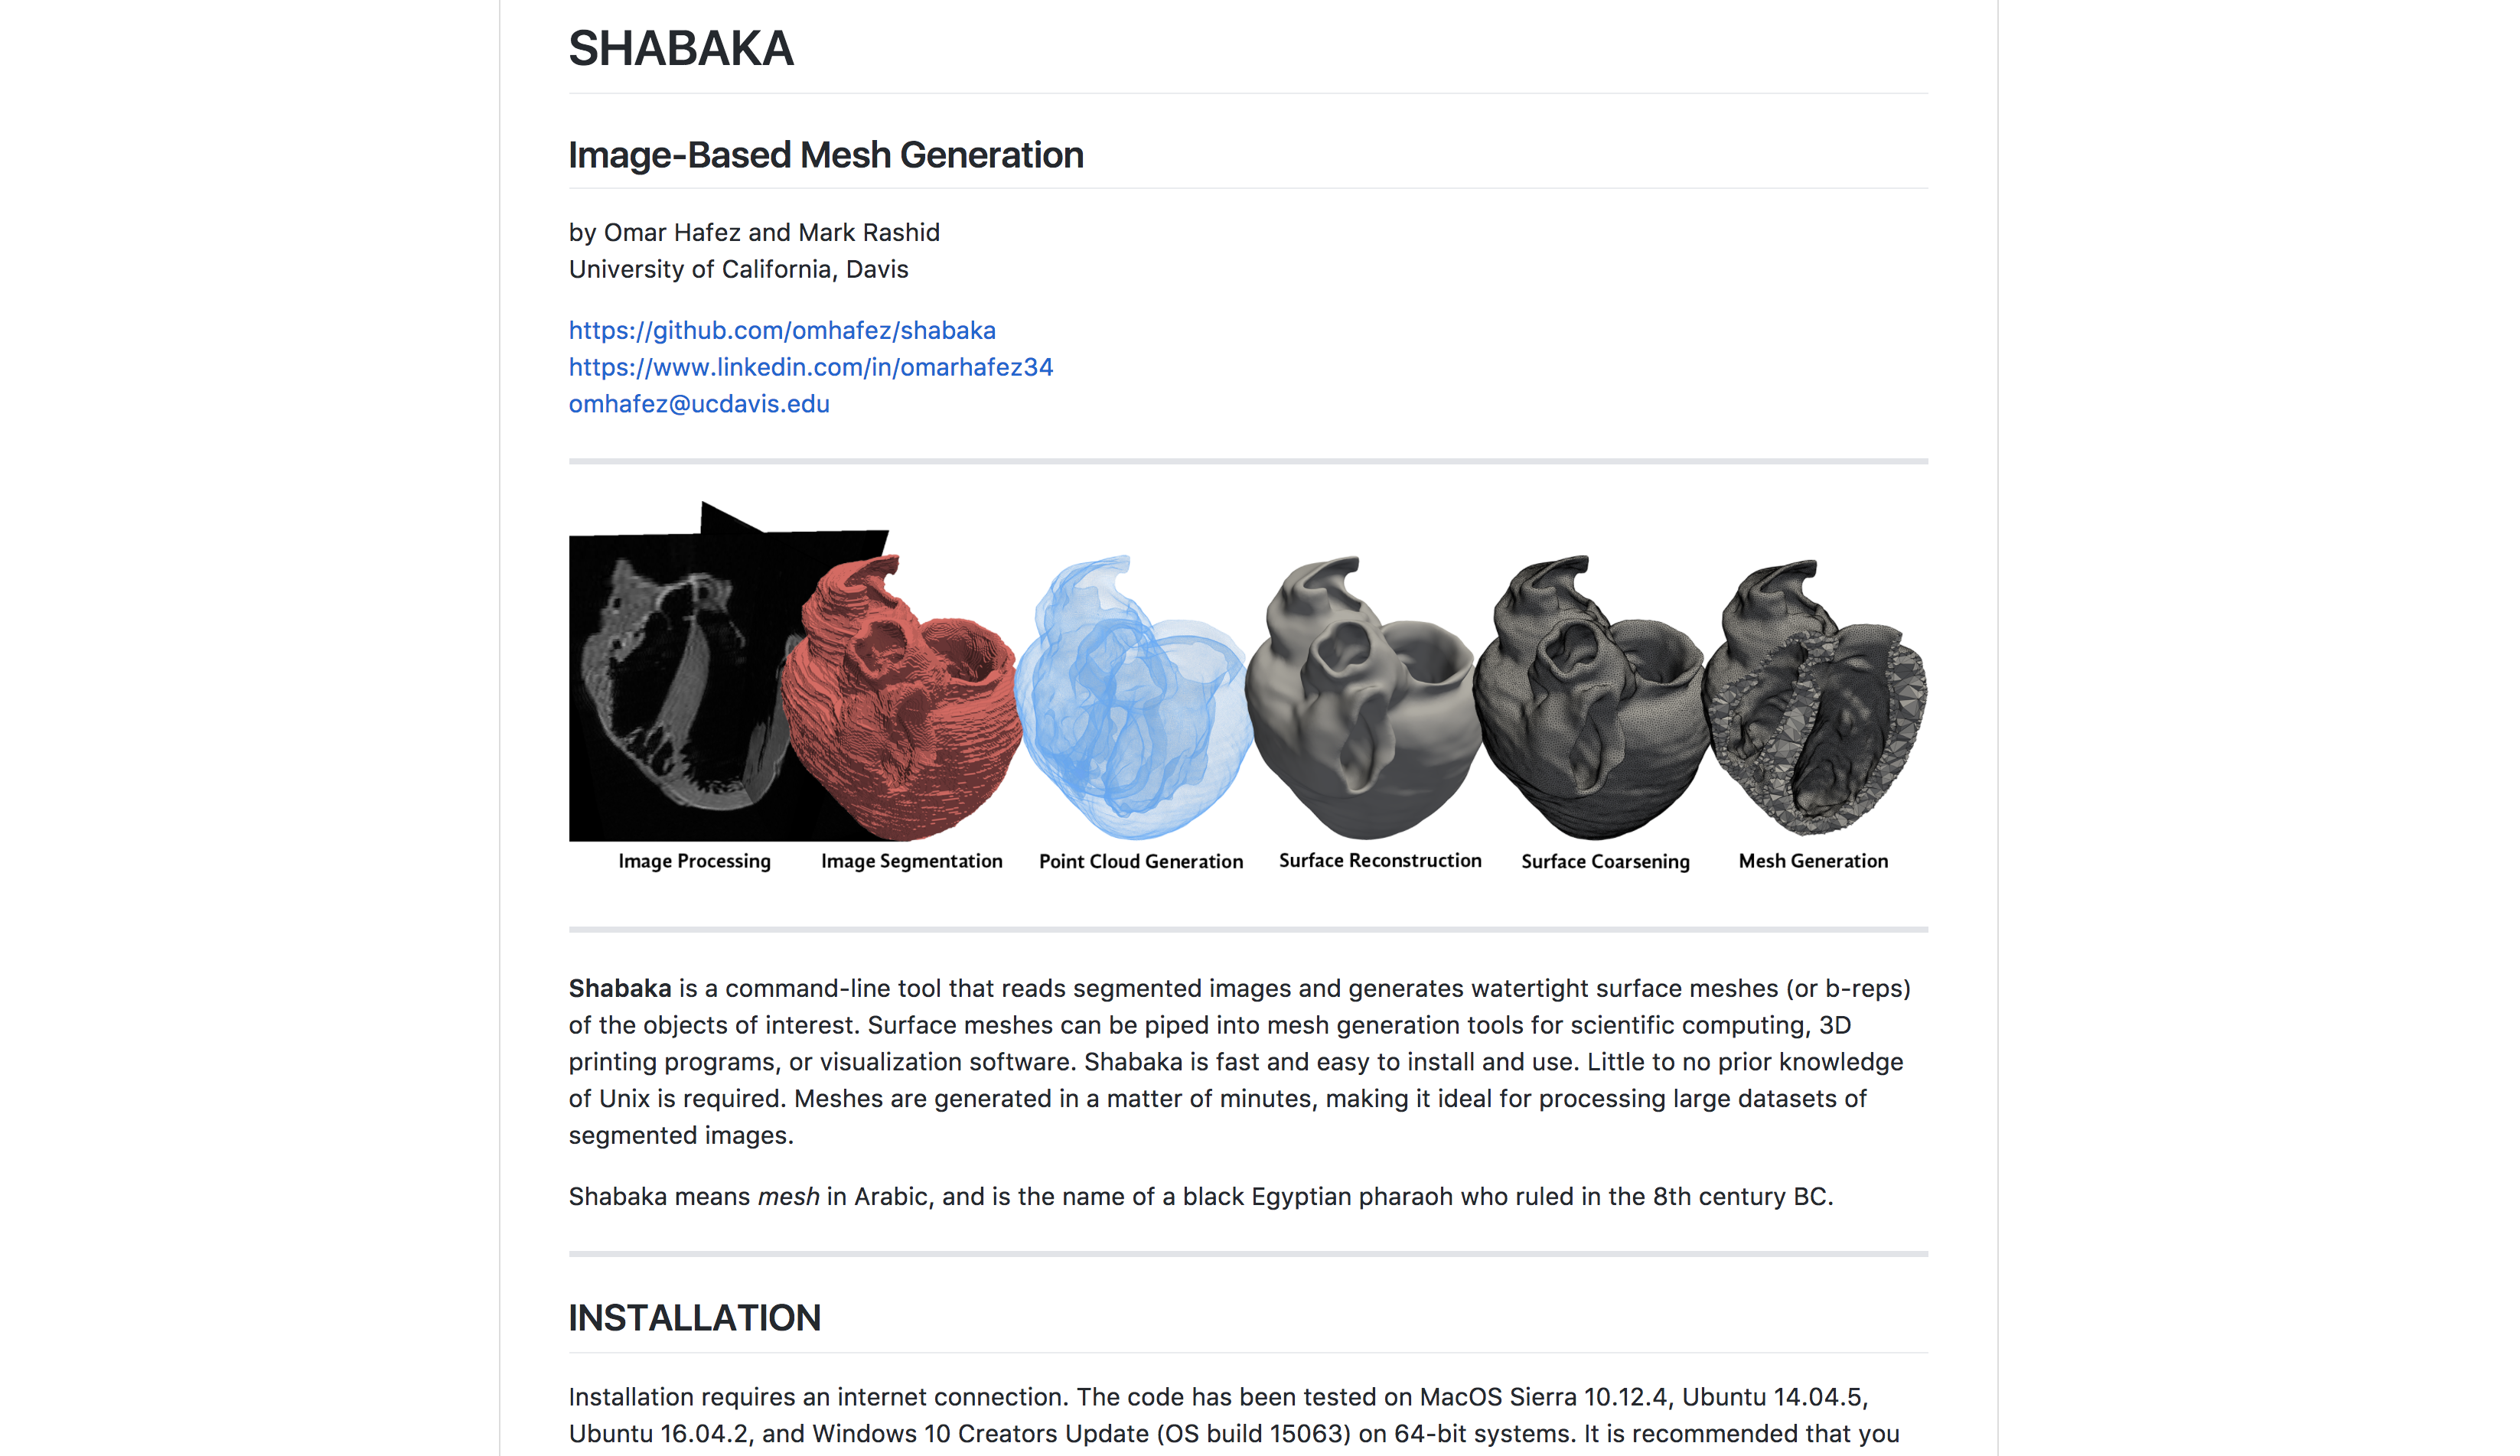
\includegraphics[width=1.0\textwidth]{media/2-shabaka/2-surf/7-shabaka.png}
\caption{Screenshot of Github repo}
\label{fig:github}
\end{figure}

%%%%%%%%%%%%%%%%%%%%%%%%%%%%%%%%%%%%%%%%%%%%%%%
%%%%%%%%%%%%%%%%%%%%%%%%%%%%%%%%%%%%%%%%%%%%%%%
\subsection{File Formats}
\label{File Formats-SURF}


\section{Mesh Generation}
%

%%%%%%%%%%%%%%%%%%%%%%%%%%%%%%%%%%%%%%%%%%%%%%%
%%%%%%%%%%%%%%%%%%%%%%%%%%%%%%%%%%%%%%%%%%%%%%%
\subsection{Hexahedral and Hex-Dominant Meshing}
\label{Hexahedral and Hex-Dominant Meshing}

%%%%%%%%%%%%%%%%%%%%%%%%%%%%%%%%%%%%%%%%%%%%%%%
%%%%%%%%%%%%%%%%%%%%%%%%%%%%%%%%%%%%%%%%%%%%%%%
\subsection{Tetrahedral Meshing}
\label{Tetrahedral Meshing}

%%%%%%%%%%%%%%%%%%%%%%%%%%%%%%%%%%%%%%%%%%%%%%%
%%%%%%%%%%%%%%%%%%%%%%%%%%%%%%%%%%%%%%%%%%%%%%%
\subsection{Polyhedral Meshing}
\label{Polyhedral Meshing}


\begin{figure}[ht]
\centering
\subfigure[]{%
		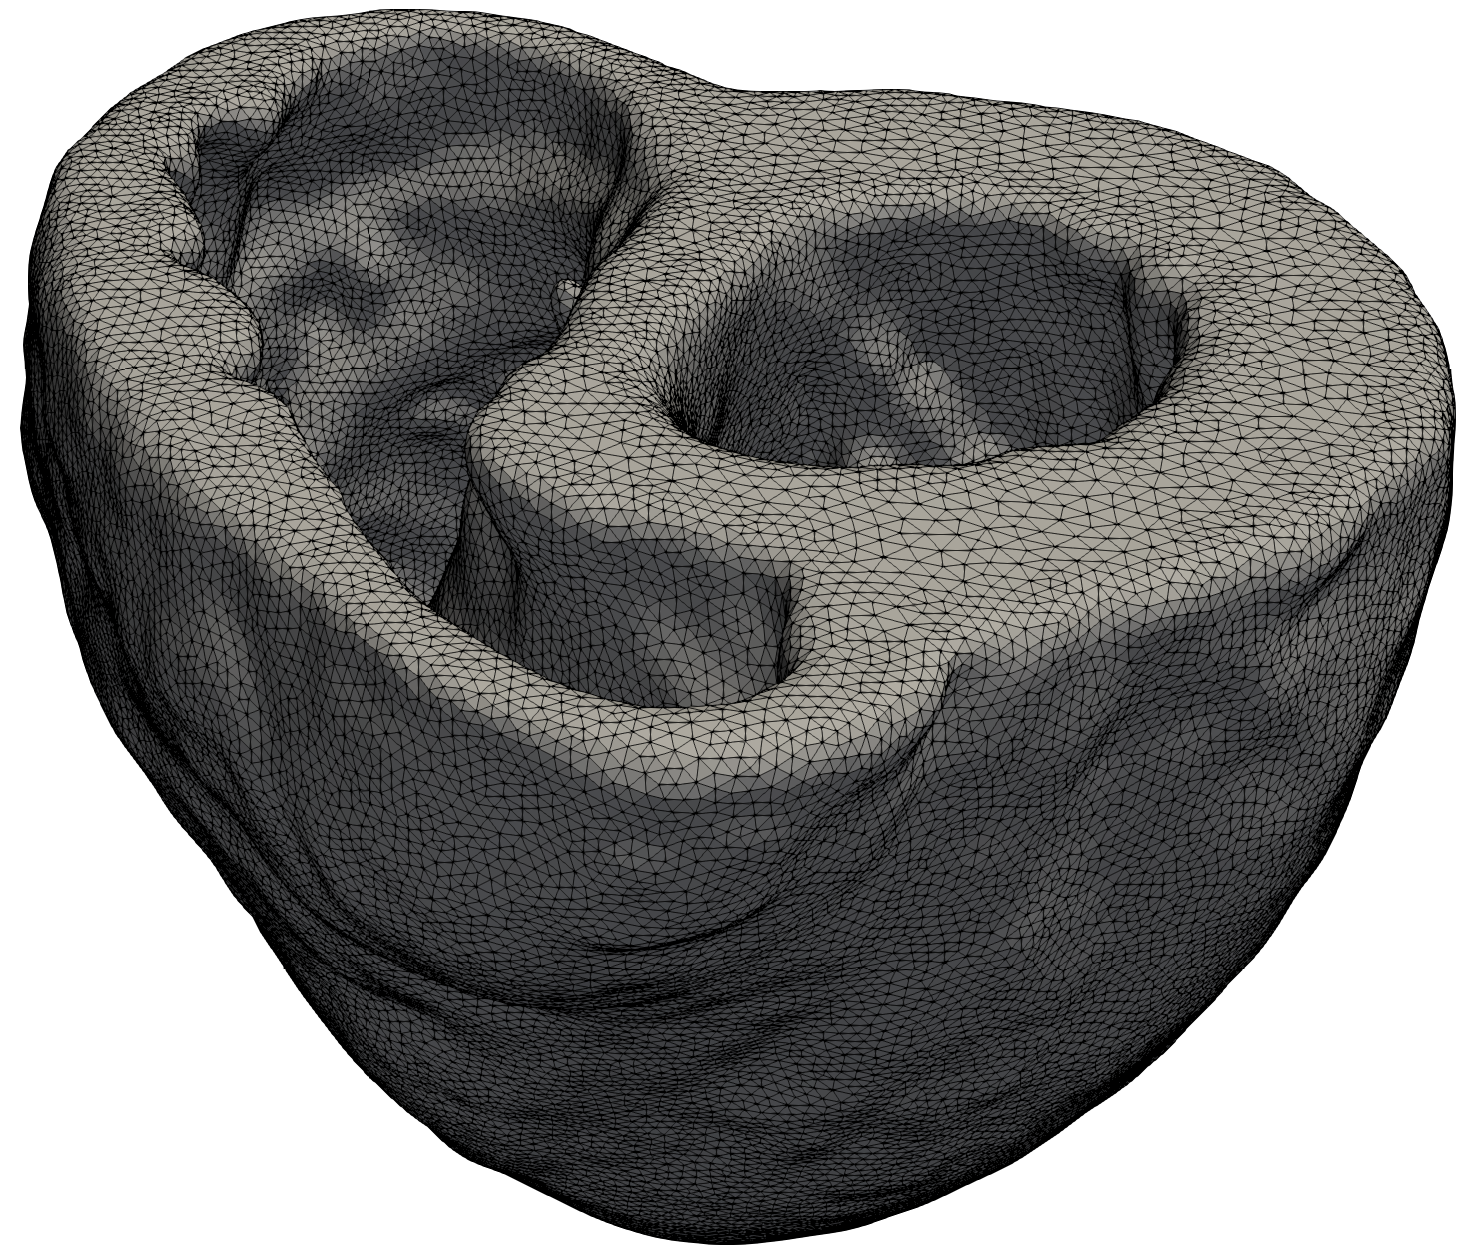
\includegraphics[scale=0.14]{media/4-cardioid/0-ventriclesurf.png}
\label{fig:tet1}}
\subfigure[]{%
		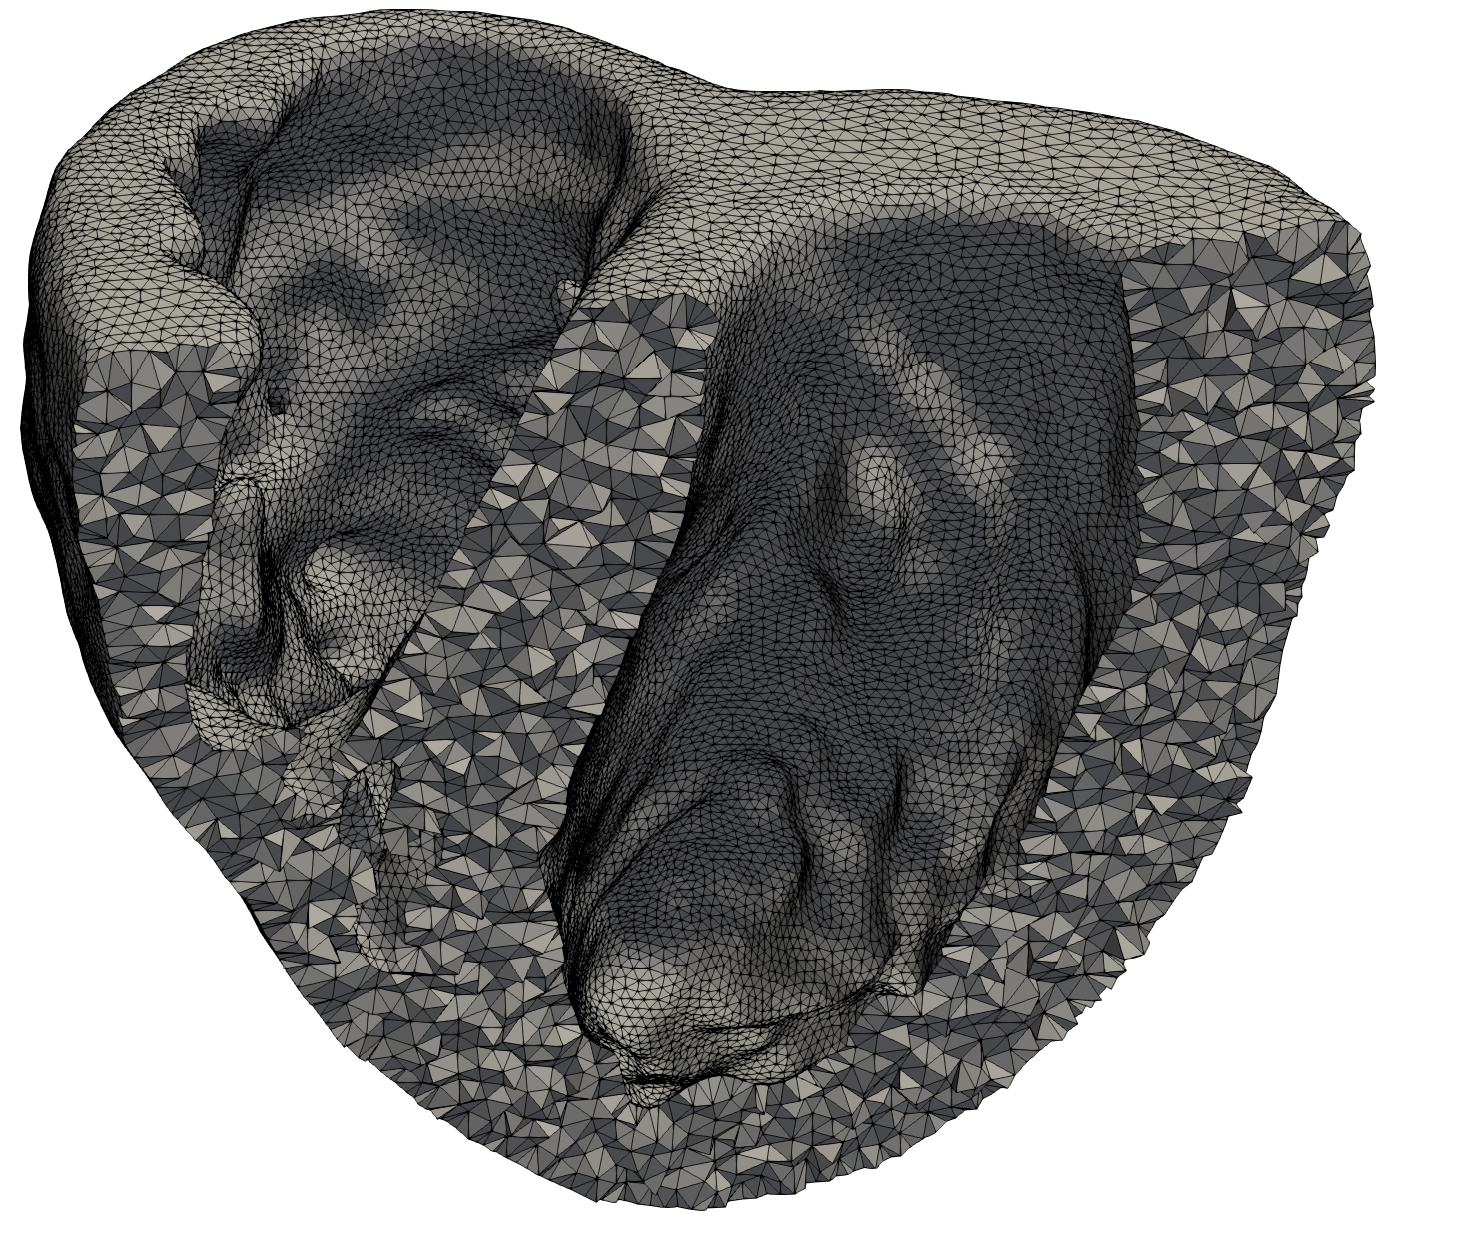
\includegraphics[scale=0.14]{media/4-cardioid/1-tet.png}
\label{fig:tet2}}
%
\caption{Bi-ventricular mesh: (a) surface mesh, and (b) clipped view of quadratic tetrahedral mesh used in Cardioid simulations}
\label{fig:tetmesh}
\end{figure}

\begin{figure}[ht]
\centering
\subfigure[]{%
		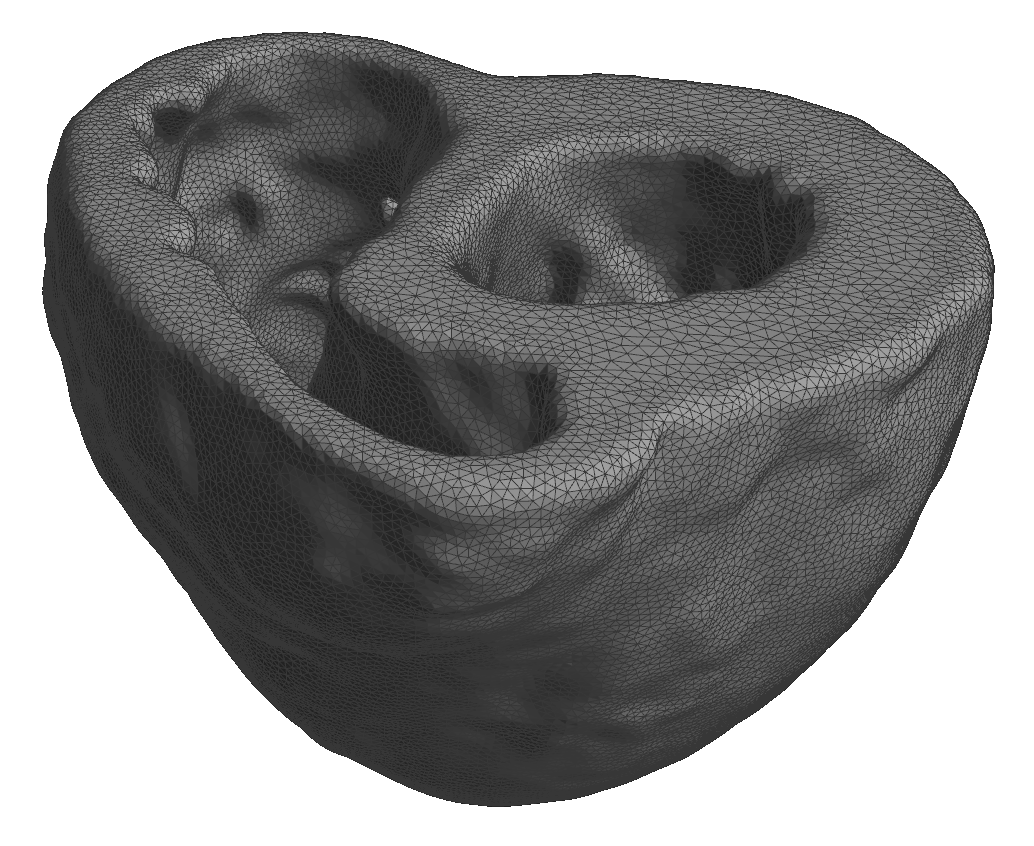
\includegraphics[scale=0.18]{media/3-celeris/1-brep.png}
\label{fig:cel1}}		
\subfigure[]{%
		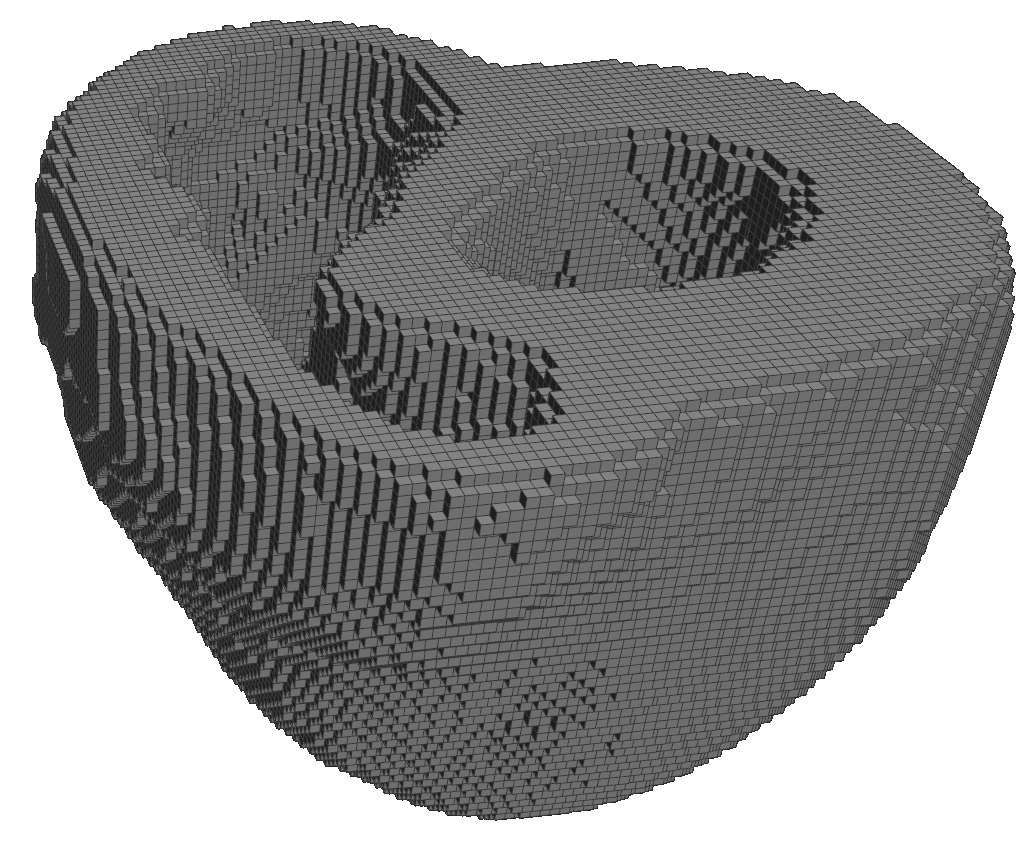
\includegraphics[scale=0.18]{media/3-celeris/2-hex.png}
\label{fig:cel2}}		
\subfigure[]{%
		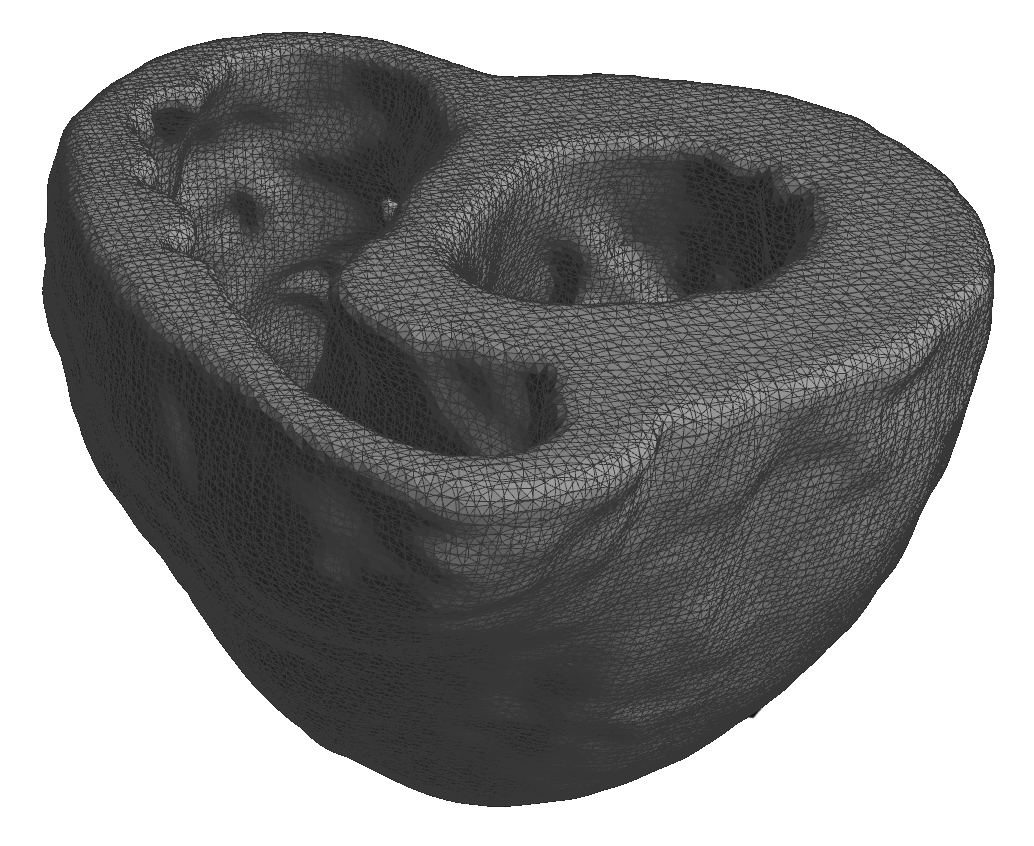
\includegraphics[scale=0.18]{media/3-celeris/3-pmesh.png}
\label{fig:cel3}}		
\subfigure[]{%
		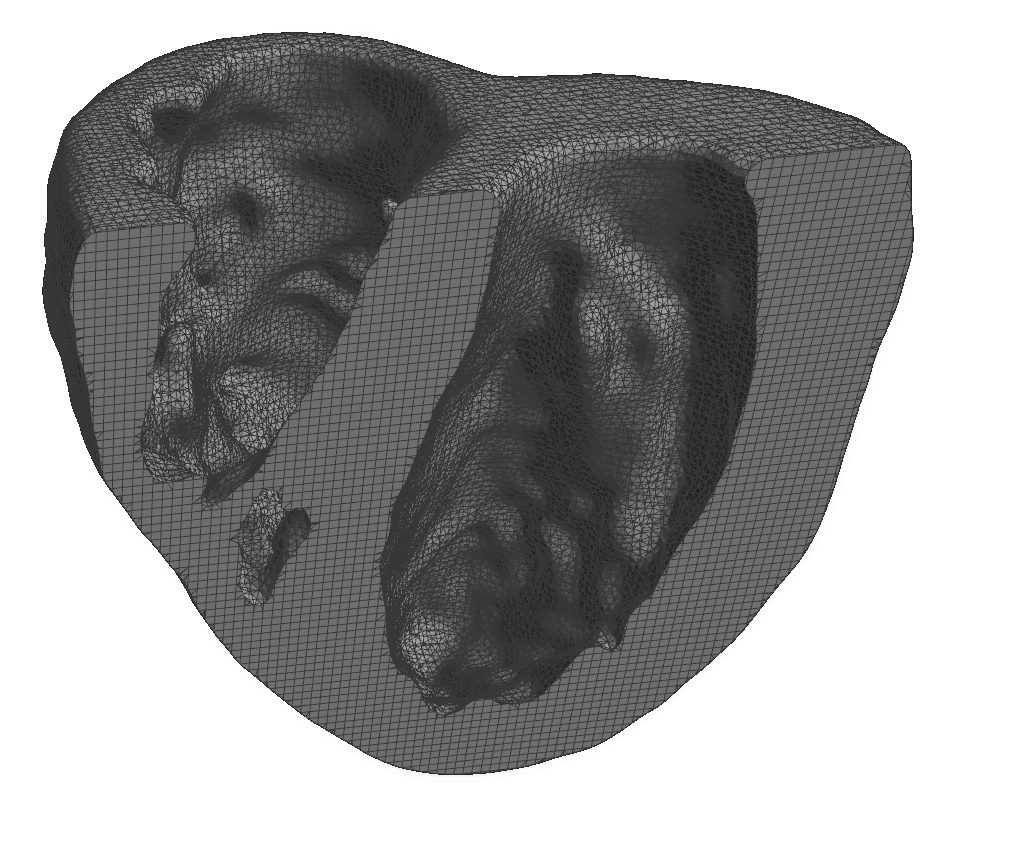
\includegraphics[scale=0.18]{media/3-celeris/4-clip.png}
\label{fig:cel4}}	
\subfigure[]{%
		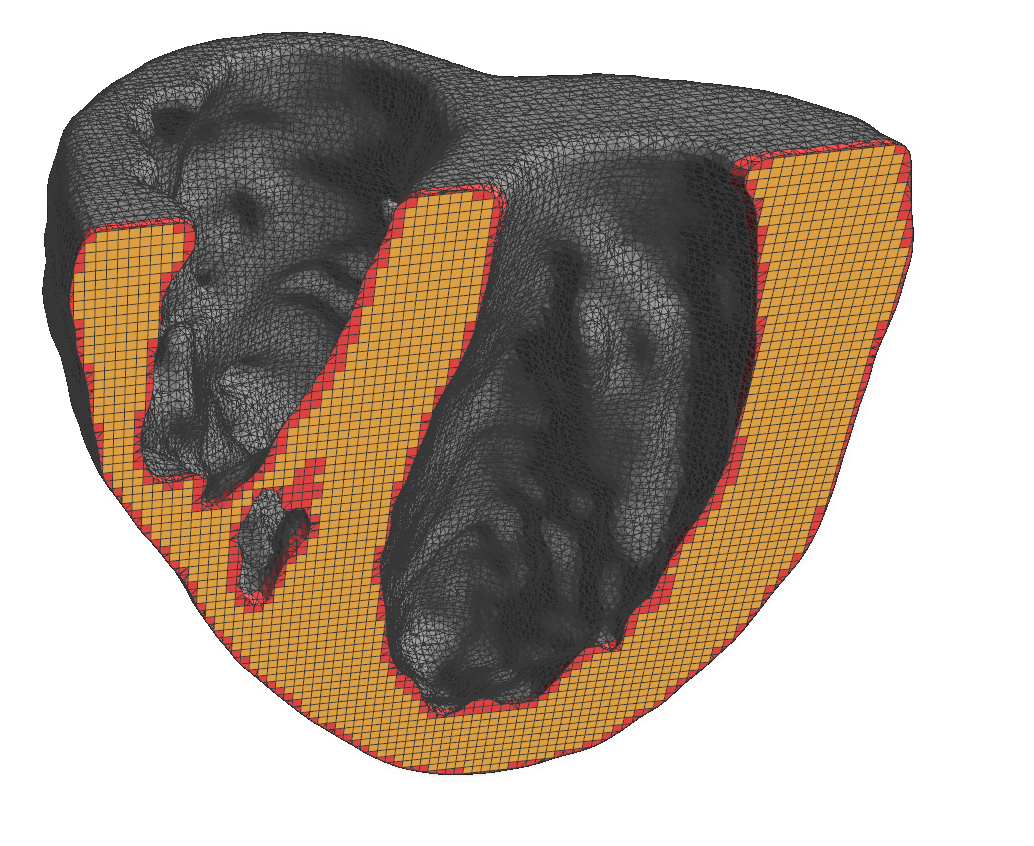
\includegraphics[scale=0.18]{media/3-celeris/5-color.png}
\label{fig:cel5}}			

\caption{Generation of polyhedral mesh: (a) input surface mesh, (b) bounding hex mesh,  (c) resulting polyhedral mesh, (d) clipped mesh, and (e) highlight of elements with cuboidal vs. general polyhedral shape.}
\label{fig:cel}
\end{figure}

\begin{figure}[ht]
\centering
\subfigure[]{%
		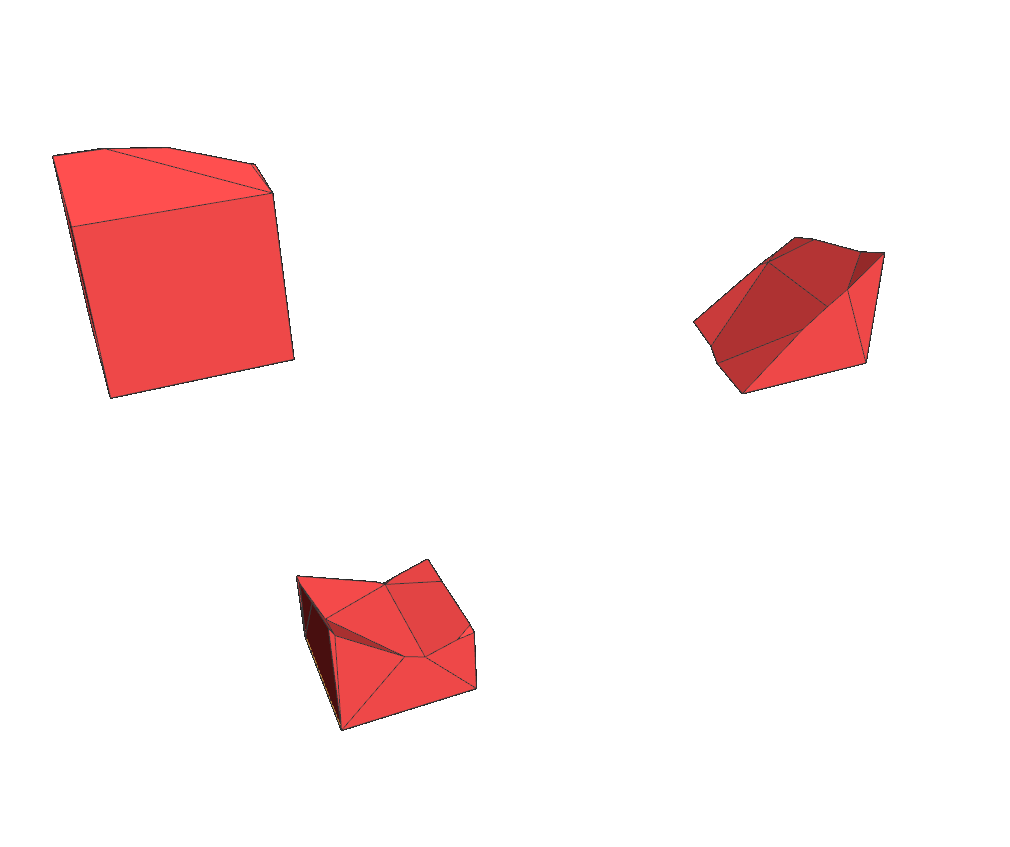
\includegraphics[scale=0.125]{media/3-celeris/zoom/zoom1.png}
\label{fig:zoom1}}		
\subfigure[]{%
		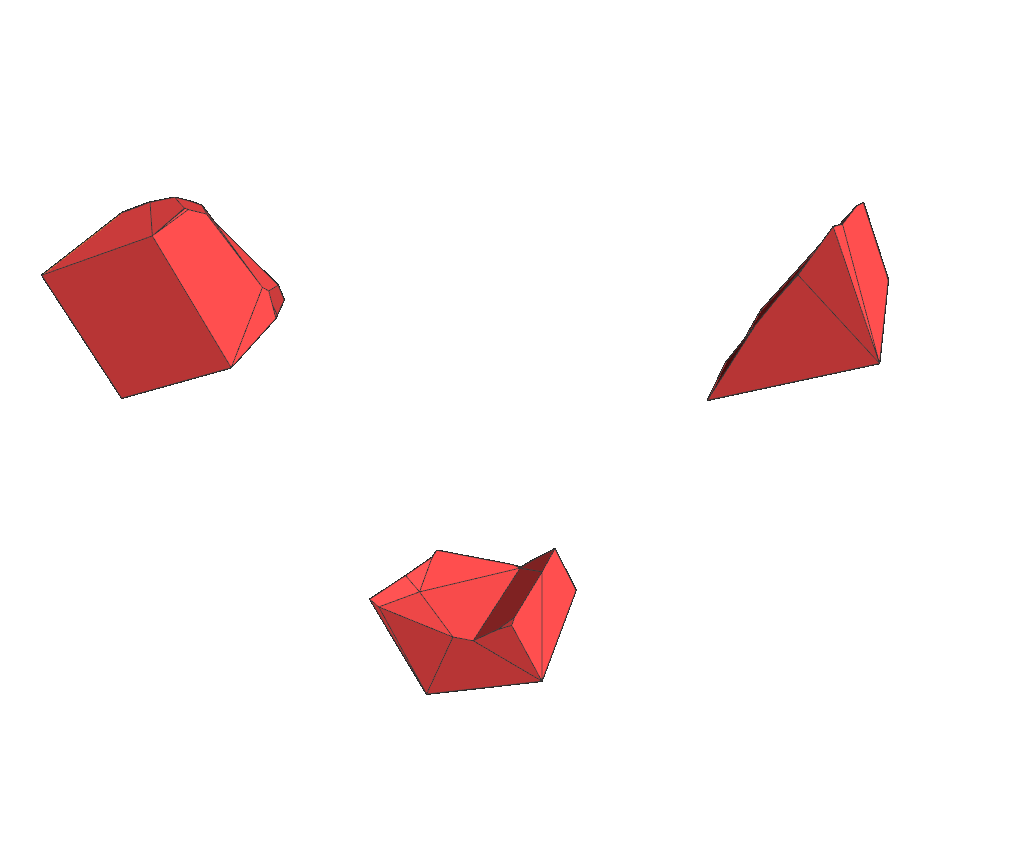
\includegraphics[scale=0.125]{media/3-celeris/zoom/zoom2.png}
\label{fig:zoom2}}		
\subfigure[]{%
		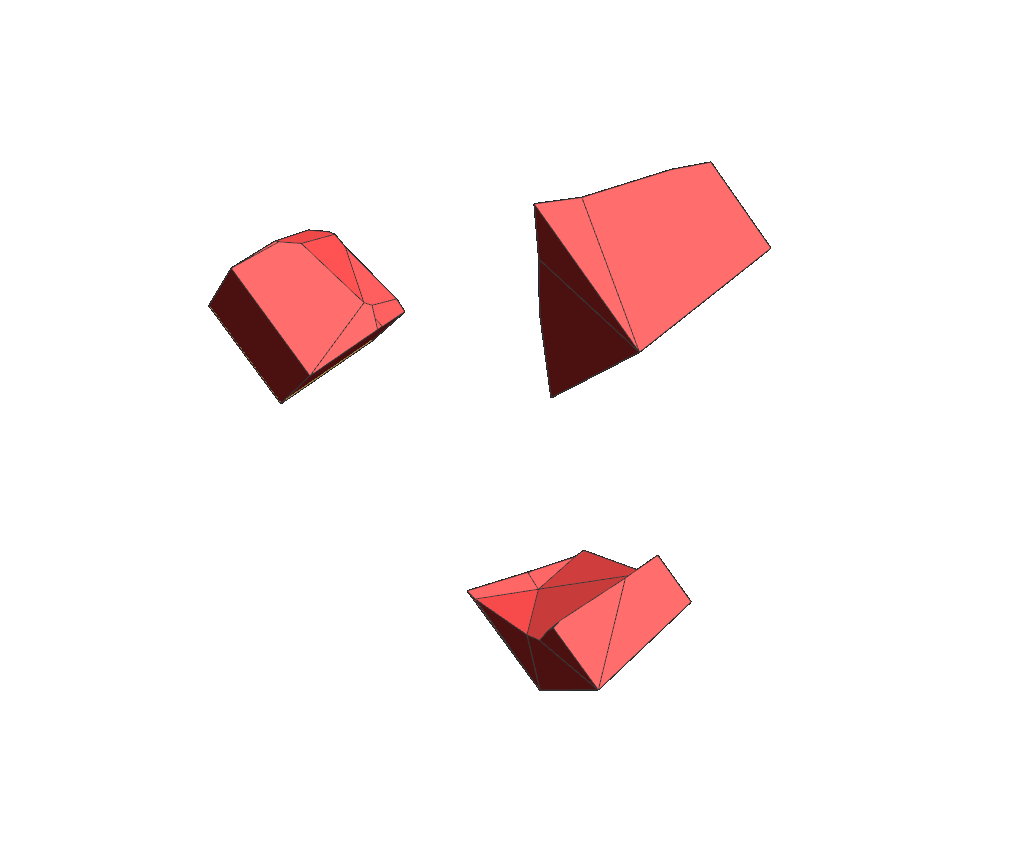
\includegraphics[scale=0.125]{media/3-celeris/zoom/zoom3.png}
\label{fig:zoom3}}		
\subfigure[]{%
		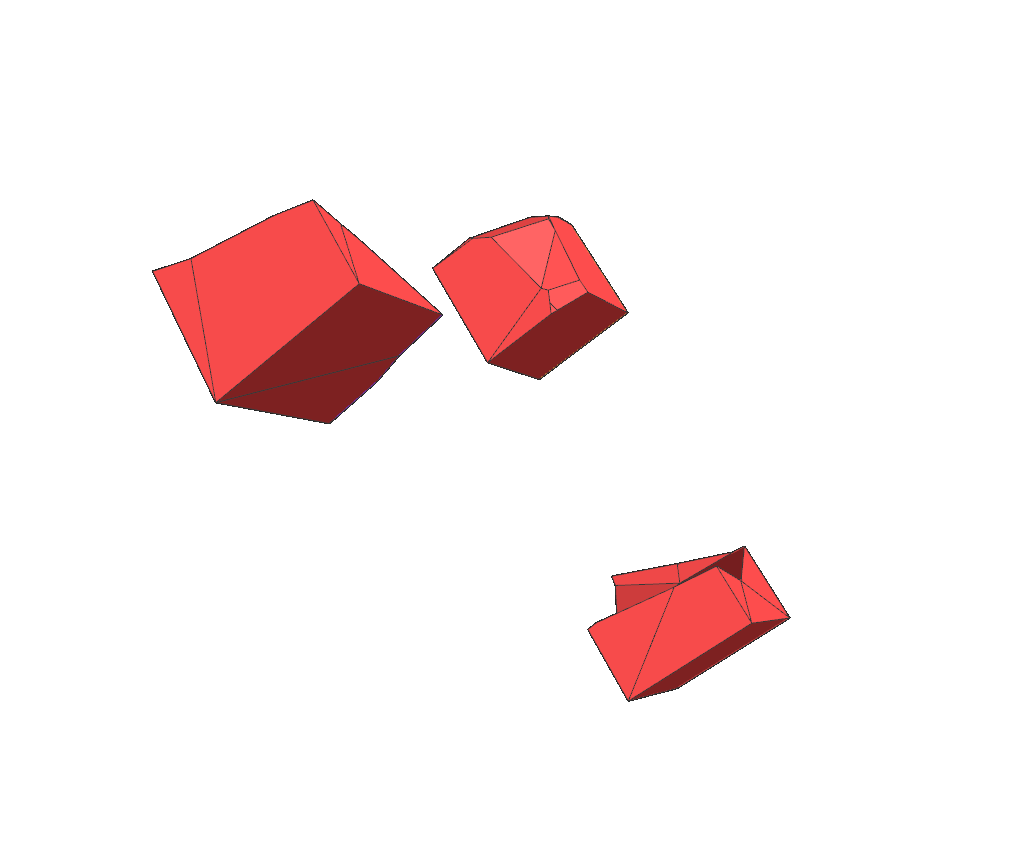
\includegraphics[scale=0.125]{media/3-celeris/zoom/zoom4.png}
\label{fig:zoom4}}	
\subfigure[]{%
		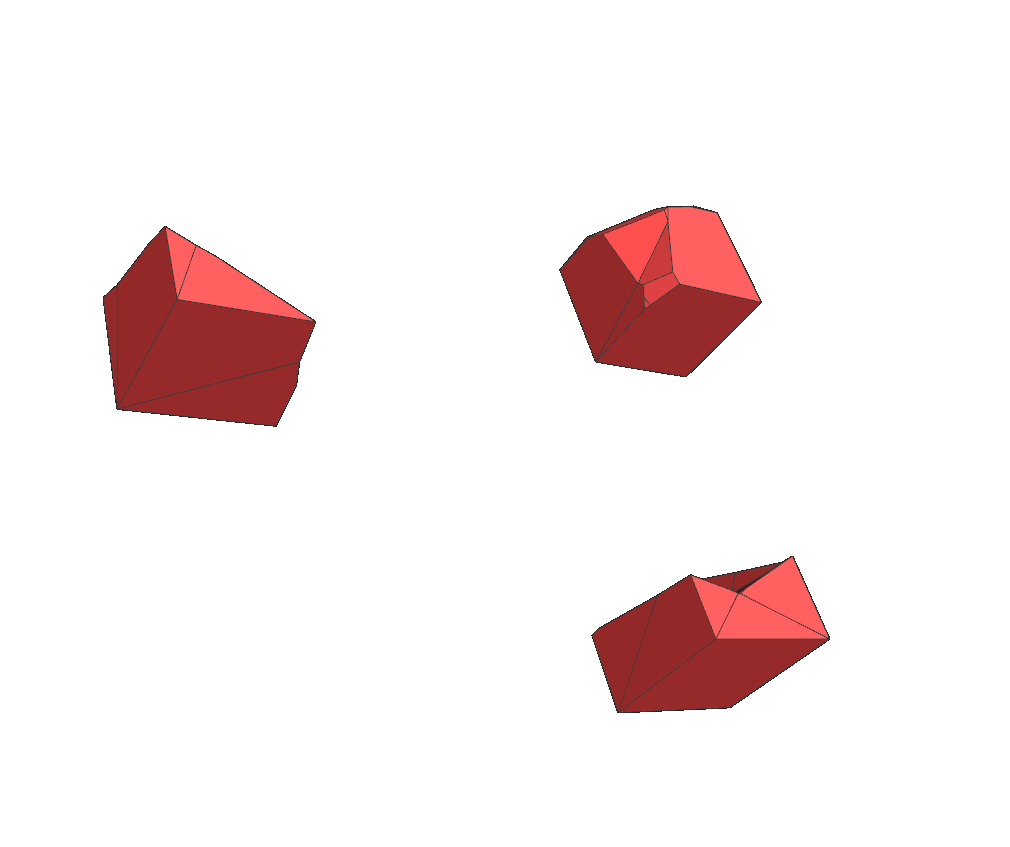
\includegraphics[scale=0.125]{media/3-celeris/zoom/zoom5.png}
\label{fig:zoom5}}		
\subfigure[]{%
		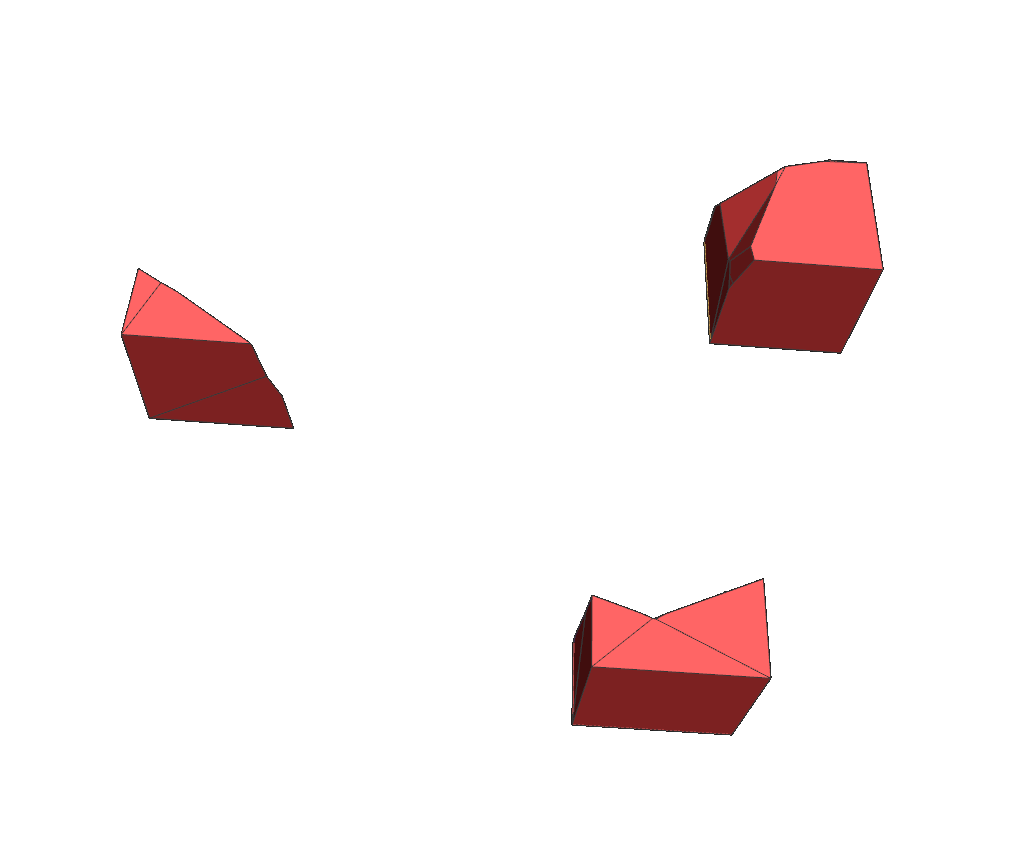
\includegraphics[scale=0.125]{media/3-celeris/zoom/zoom6.png}
\label{fig:zoom6}}	

\caption{Three example arbitrary polyhedral elements presented at different angles}
\label{fig:zoom}
\end{figure}

\begin{figure}[ht]
\centering
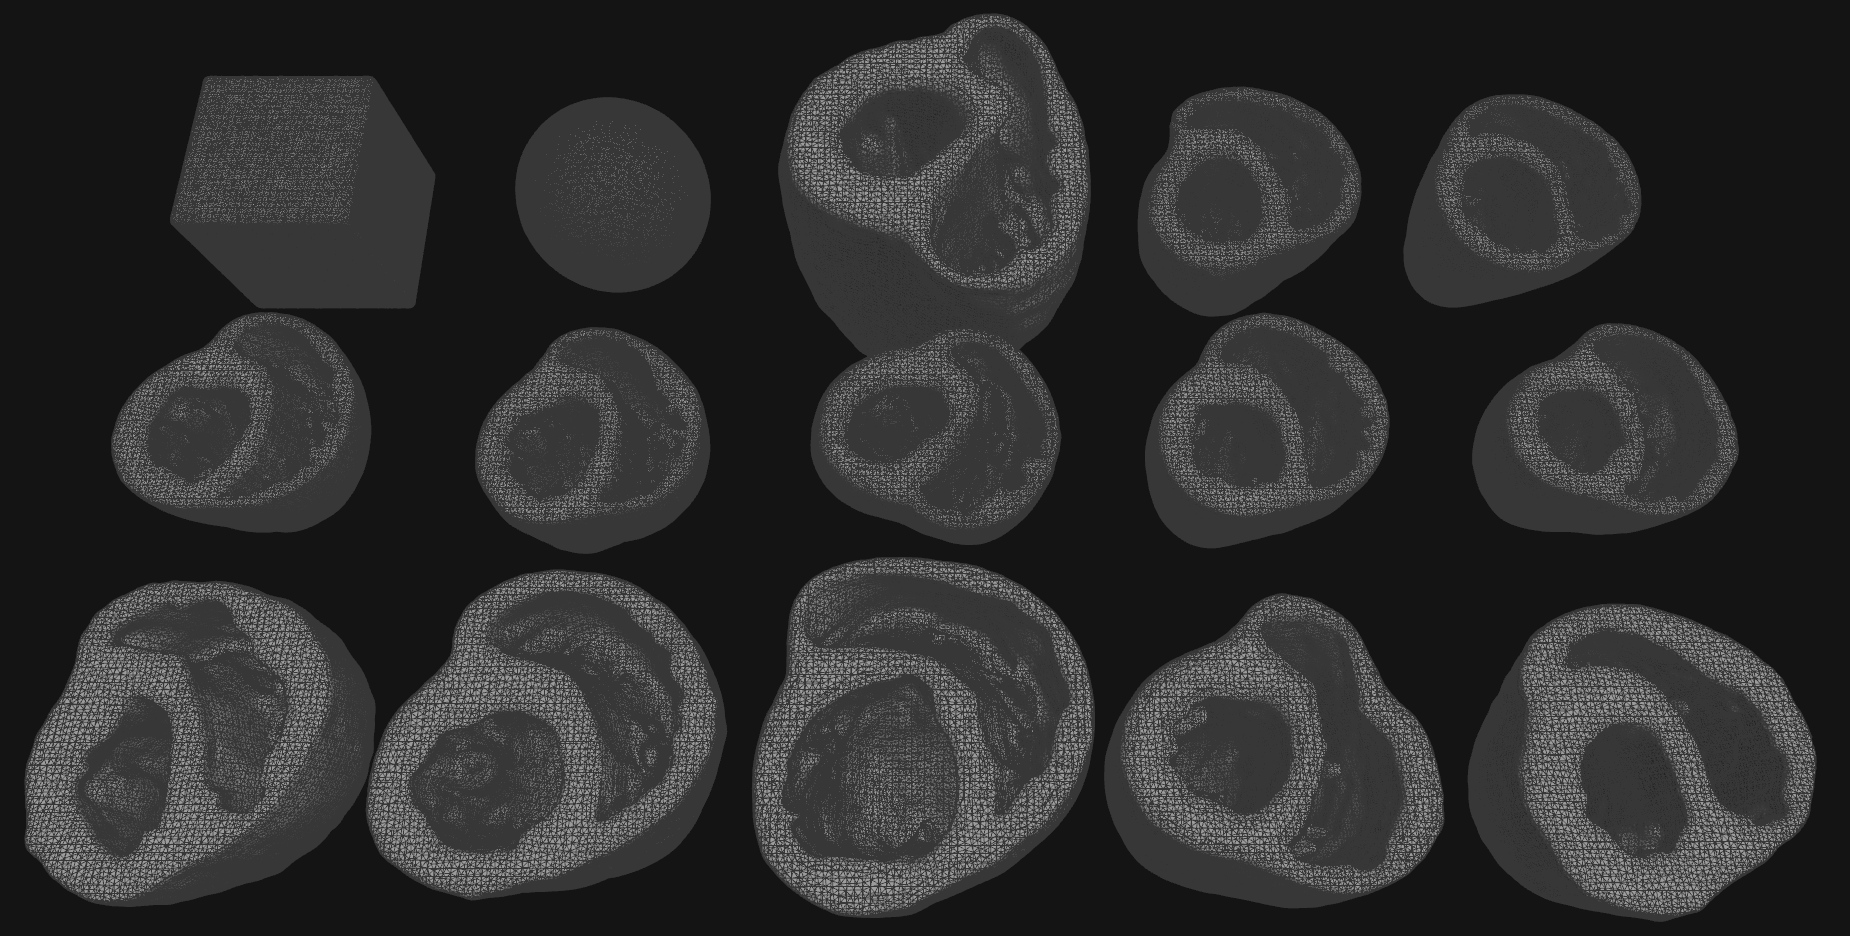
\includegraphics[width=1.0\textwidth]{media/3-celeris/7-suite.png}
\caption{Suite of polyhedral finite element meshes generated from image data \vspace{1cm}}
\label{fig:celsuite}
\end{figure}

%%%%%%%%%%%%%%%%%%%%%%%%%%%%%%%%%%%%%%%%%%%%%%%
%%%%%%%%%%%%%%%%%%%%%%%%%%%%%%%%%%%%%%%%%%%%%%%
\subsection{File Formats}
\label{File Formats-MESH}


\section{Shabaka: A Free Image-Based Meshing Tool}